% !TEX root = tjumain.tex
% !Mode:: "TeX:UTF-8"

% \iffalse
% \bibliography{reference/reference.bib} % 欺骗latextools获取bib文件
% \fi

%%%%%%% 正文 %%%%%%%
% !TEX root = ../tjumain.tex
\chapter{报告摘要}

在本次关于 TCP 的实践中,我们设计并实现了一个基于应用层和RFC 793 文档的 TCP 协议实体,能够实现包括“连接管理”(连接建立与断开)、“拥塞控制”、“可靠数据传输”等功能。同时,还对数据结构进行优化,实现在 50Mbps,6ms 延迟

  
% !TEX root = ../tjumain.tex

\chapter{总体设计}

根据TCP协议具有的功能和实践内容结合,本次实验的协议设计分为以下三个部分,分别是连接管理和流量控制、可靠数据传输和拥塞控制。

\section{可靠数据传输相关设计}

为了向应用层提供可靠的端到端数据传输服务。我们需要有 连接建立、数据传输、连接关闭 三个方面的功能。在本次实验中,我们首先在第一周完成了连接建立的过程,即通过三次握手完成 TCP 连接的建立。本周,我们将重点完成第二个功能,即可靠的数据传输服务。

相关的API如下:
\begin{enumerate}
  \item Client \begin{enumerate}
    \item int tju\_send(...): 将应用层的信息放入发送缓冲区,并进行发送。
  \end{enumerate}
  \item Server \begin{enumerate}
    \item int tju\_recv(...): 接收由 handle\_packet 等函数放入接收缓冲区的信息
  \end{enumerate}
  \item 通用 \begin{enumerate}
      \item tju\_tcp\_t * tju\_socket(): 创建 socket 并初始化数据结构(包括发送、接收缓冲区等),根据本周的要求,还增加了关于时钟初始化、trace 文件初始化等操作,最终返回 socket 的指针
      \item tju\_handle\_packet(): 处理接收到的包裹。在 Established 状态下,根据接收缓冲区的大小,选择性的将不按顺序到来的包裹放入接收树(自定义数据结构)或者丢弃。并在接收到正确包裹时,将树中正确的包裹按顺序放入缓冲区中等待应用层获取。
  \end{enumerate}
\end{enumerate}

\section{模块功能设计}

\begin{figure}[!htbp]
  \centering
  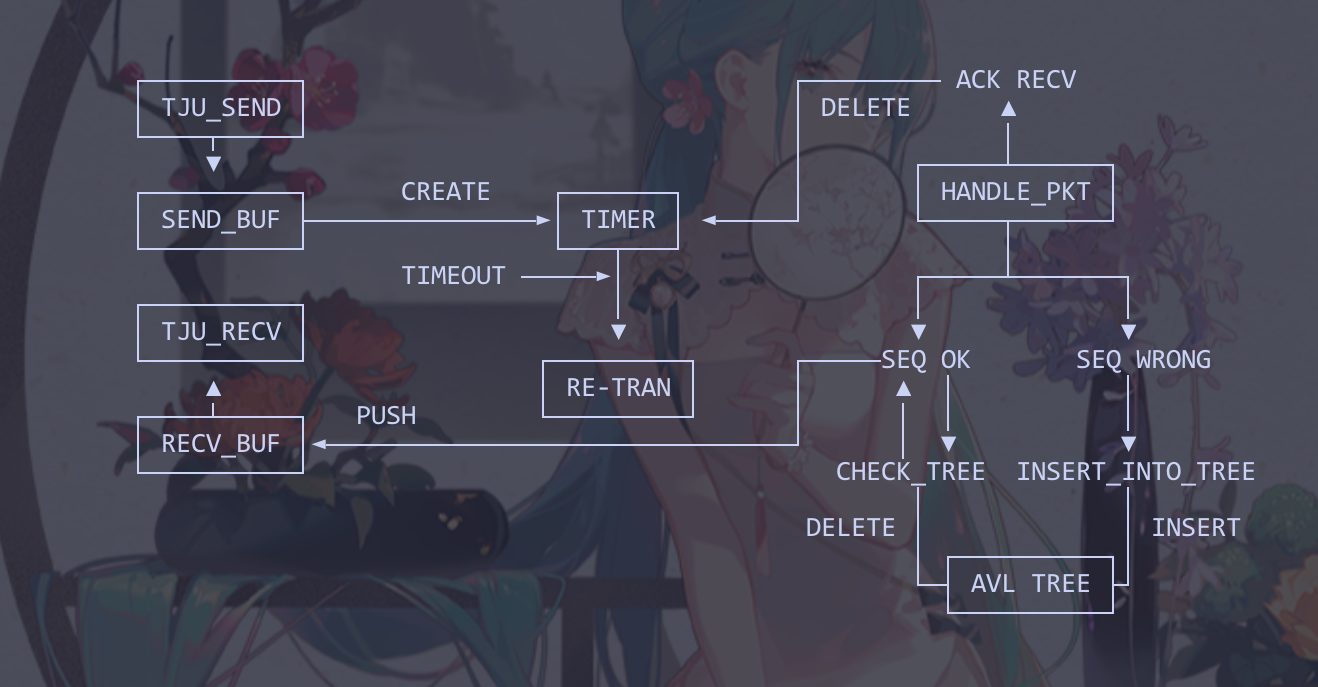
\includegraphics[width=.8\textwidth]{figures/Flow_10_4.png}
  \label{fig:flow}\caption{可靠数据传输相关功能设计总览}
\end{figure}

从图中可以看到,我们通过一个 TIMER 线程专门检查所有 registered TIMER 并在其 TIMEOUT 时执行 RE-TRAN,即重传。同时,我们在 HANDLE\_PACKET 函数,在收到 ACK 时,关闭响应的 TIMER(TIMER的实现采用 queue 的数据结构,确保快速增删)。

对于 Server 端,我们在 HANDLE\_PACKET 中设计了根据 SEQ number 的检验功能,当 SEQ number 正确时,我们直接将内容放入缓冲区,否则将其放入一颗 AVL 树中等待正确 SEQ 达到后,再进行查找并放入缓冲区,确保缓冲区中的内容都是连贯一致的。



% !TEX root = ../tjumain.tex

\chapter{连接建立的设计}
该部分涉及到的TCP的状态转变如下图\ref{fig:fsm}所示:

\section{状态机设计}

TCP 可靠数据传输过程如下所示,对于出现丢包的情况,在 Client 端采用重传机制,不在 Server 端关于 ACK 丢掉的处理机制。同时,在 Server 端采用了 AVL Tree 的数据结构存储乱序到达的数据包,确保最终呈现在接收缓冲区的内容是有序的。

\subsection{Client 端状态机设计}

\begin{figure}[!htbp]
    \centering
    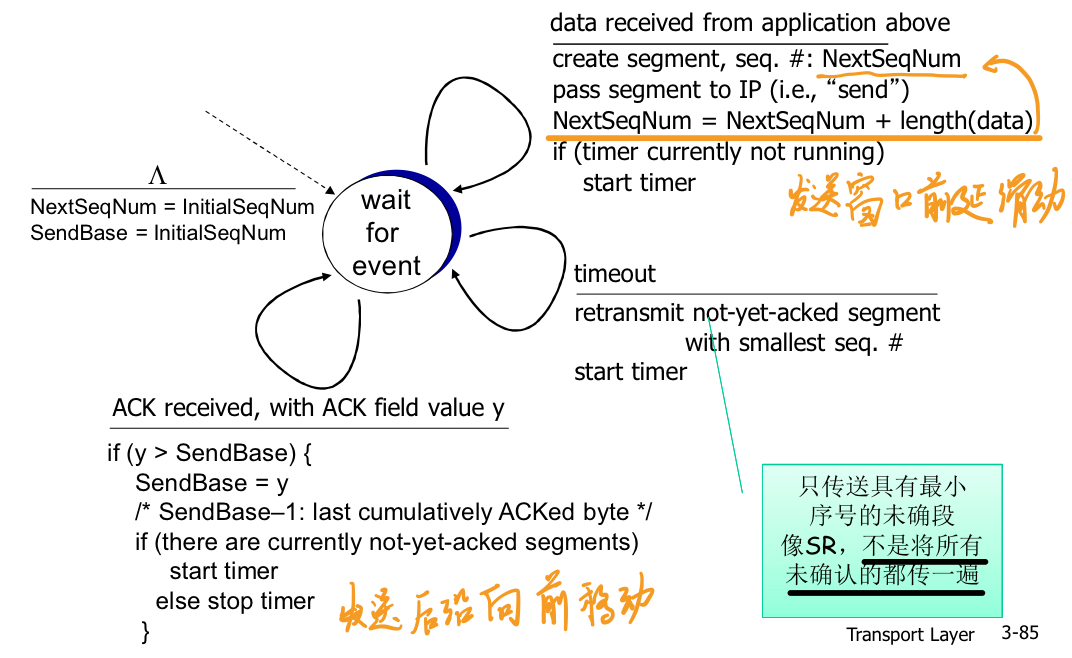
\includegraphics[width=.8\textwidth]{figures/CLIENT_FSM.png}
    \label{fig:client_fsm}\caption{Client FSM}
  \end{figure}

Client 端状态机如图\ref{fid:client_fsm}所示。Client 端需要响应三种事件:
\begin{enumerate}
    \item 来自上层的调用,将数据打包并发送给下一层实体(toLayer3),然后新建 TIMER 并 注册之
    \item 来自TIMEOUT 通过 TIMER 的信息进行超时重传(需要调整一下rtt等信息)
    \item 收到 ACK,确认 ACK 的状态,根据 ACK 信息选择性地关闭 TIMER 
\end{enumerate}

\subsection{Server 端状态机设计}

\begin{figure}[!htbp]
    \centering
    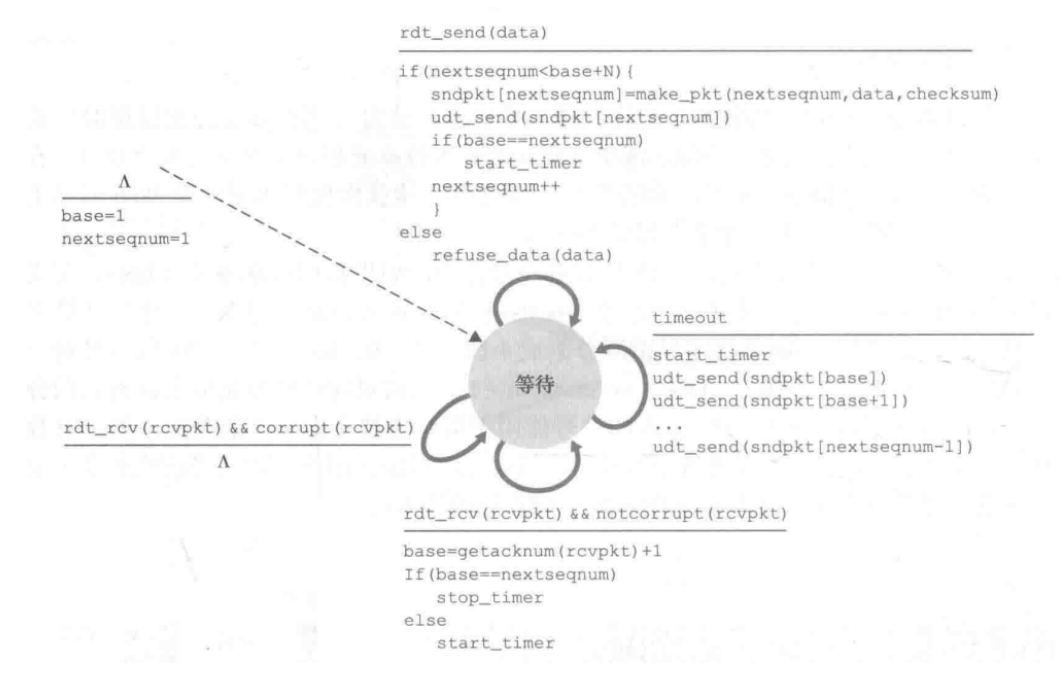
\includegraphics[width=.8\textwidth]{figures/SERVER_FSM.png}
    \label{fig:server_fsm}\caption{Server FSM}
  \end{figure}

在 Server 端,我们目前暂不考虑数据出错的情况,即达到的包,都是正确的。在此情况下,我们需要处理一下情况:


\begin{enumerate}
    \item 到达SEQ正确:判断缓冲区大小,选择性的将其放入缓冲区,发送ACK。同时在AVL中递归地查找连续的正确的包裹
    \item 到达SEQ大了:将其放入 AVL Tree 并发送ACK
    \item 到达SEQ小了:收到过,丢弃
\end{enumerate}

\section{超时重传机制}

\paragraph*{连接建立时} 丢失有三种:第一次握手丢失,服务端返回第二次握手丢失,以及第三次确认丢失。第一、二个由 Client 端设置定时器保护,第三个由 Server 端设置定时器保护,即当收到第三次确认时,Server 端再将信息定时器进行关闭。

\paragraph*{发送数据时} 丢失有两种:发送数据丢失(Seq),发送ACK丢失。二者对于 Client 端的表现均是长时间(RTO)没收到 ACK 信息,于是我们将定时器设置在 Client 端,由 Client 端进行超时重传。而 Server 只对于前者,即发送数据丢失的情况作出反馈,即设置乱序到达,顺序提交的机制,确保因超时而呈现乱序到达的数据得以顺序提交给上层用户。

\section{RTO 计算法则}

RTO 是超时重传机制的基础。由于网络变化,RTO应当是动态调整的。如果TCP 过早重传,会导致注入多数不必要的报文,阻塞网络。如果过晚重传,则会影响网络使用效率。我们根据 RFC793 的标准,让Socket维护了一个 SampleRTT均值(EstimatedRTT)通过如下公式进行更新:
\begin{equation}
    EstimatedRTT := (1-\alpha)\times EstimatedRTT + \alpha\times SampleRTT
\end{equation}\label{eq:est}

除了RTT,RFC 6298 还定义了 RTT 的偏差 DevRTT 的计算,用于usuan SampleRTT 和EstimatedRTT 的偏离程度
\begin{equation}
    DevRTT := (1-\beta)\times DevRTT + \beta\times|SampleRTT - EstimatedRTT|
\end{equation}
于是,最终的TRO计算公式如下:
\begin{equation}
    RTO := EstimatedRTT + 4\times DevRTT
\end{equation}\label{eq:rto}

\section{流量控制}

流量控制也是 TCP 标准功能之一,是构成可靠传输的关键步骤,能够与其他 TCP 实体一起,维护整个网络的传输可靠性。如果流量过大,则会导致接收方不断丢弃传输的结果,发送方不断进行重发。故而,Server 端需要将rwnd的信息通过 ACK 信息携带给 Client 端,让 Client 能够正确地调整发送速率。

% !TEX root = ../tjumain.tex
\chapter{协议实现部分}

首先,从宏观上阐释:我们TCP实现部分采用了两个线程进行服务:发送线程和接收线程。

\paragraph*{发送线程} 负责从数据结构 sending\_queue 中取出并按需发送报文、设置时钟,检查时钟进行超时重传。在用户调用 tju\_socket 生成 socket 时创建。首先发送线程会到达 ACK 时预订消除的时钟进行 删除,然后判断是否有超时时钟,执行重传。最后进行正常报文的发送。

\paragraph*{接收线程} 负责从socket中获取对方发送的报文、返回 ACK 并处理不按需到达的报文,确保放入 recv\_buf 中的数据是正确且有序的。在接收线程收到包裹后,调用 tju\_handle\_packet 进行处理。

\paragraph*{tju\_handle\_packet} 处理报文的主要函数,通过 switch ,根据当前 socket 的状态选择合适分支进行报文的处理。

\section{连接建立的实现}

要实现连接的建立,我们实现了如图\ref{fig:established}的流程图。实现了 tju\_conn 和 tju\_accept 供 client 以及 server 端进行调用的 API

\paragraph*{tju\_conn} Client 端通过该 API 对Server 端发起连接请求。而后进入等待循环,直到自己 socket 的状态变为 Established 再返回。而 socket 状态的改变则由接收线程处理。

\paragraph*{tju\_accept} Server 端调用该API,从处于 LISTEN 状态的 socket 的 full\_connection 列表中获取一个全连接的 socket 即可。

\paragraph*{接收线程-三次握手}在 tju\_handle\_packet 中,关于连接建立有如下三种情况:

\begin{enumerate}
    \item LISTEN: 此状态为 Server 端。接收到 SYN 报文后,Server 端将状态变为 SYN\_RECV 并发出 SYN | ACK 报文,同时将其放入半连接队列中,发送线程需要对半连接中的sock进行重发
    \item SYN\_SENT:此状态为 Client 刚发送完 SYN 包裹,从连接的角度来说是 Client 端。此时收到包裹应为 SYN | ACK,否则拒收,由发送线程进行重发。接收正确报文后,socket 状态调整为 ESTABLISHED,同时返回一个 ACK 报文答复。
    \item SYN\_RECV:此状态为 Server 端发送完 SYN | ACK 报文,等待client的ACK。得到 ACK 后,将其半连接的sock拿出,放入全连接队列,等待 tju\_accept 进行调用。
\end{enumerate}

\section{可靠数据传输的实现}

\subsection{数据结构}

为了更好地实现可靠数据传输,我们额外实现了三种数据结构进行更优化的处理。分别是 timer\_list,queue和tree。

\paragraph*{timer\_list} 是对超时重发的处理,本质上是一个队列,其实现的头文件如图\ref{fig:timer_list}所示。对于每个 timer 我们记录了它创建的时间和创建时根据 socket RTO 计算出的 timeout 时间,以及它所代表的 tju\_packet\_t 和重传时的回调函数。我们采用 list 链表的形式进行整个线性表的遍历。当然,我们需要对其进行加锁,避免出错。

\begin{figure}[!htbp]
    \centering
    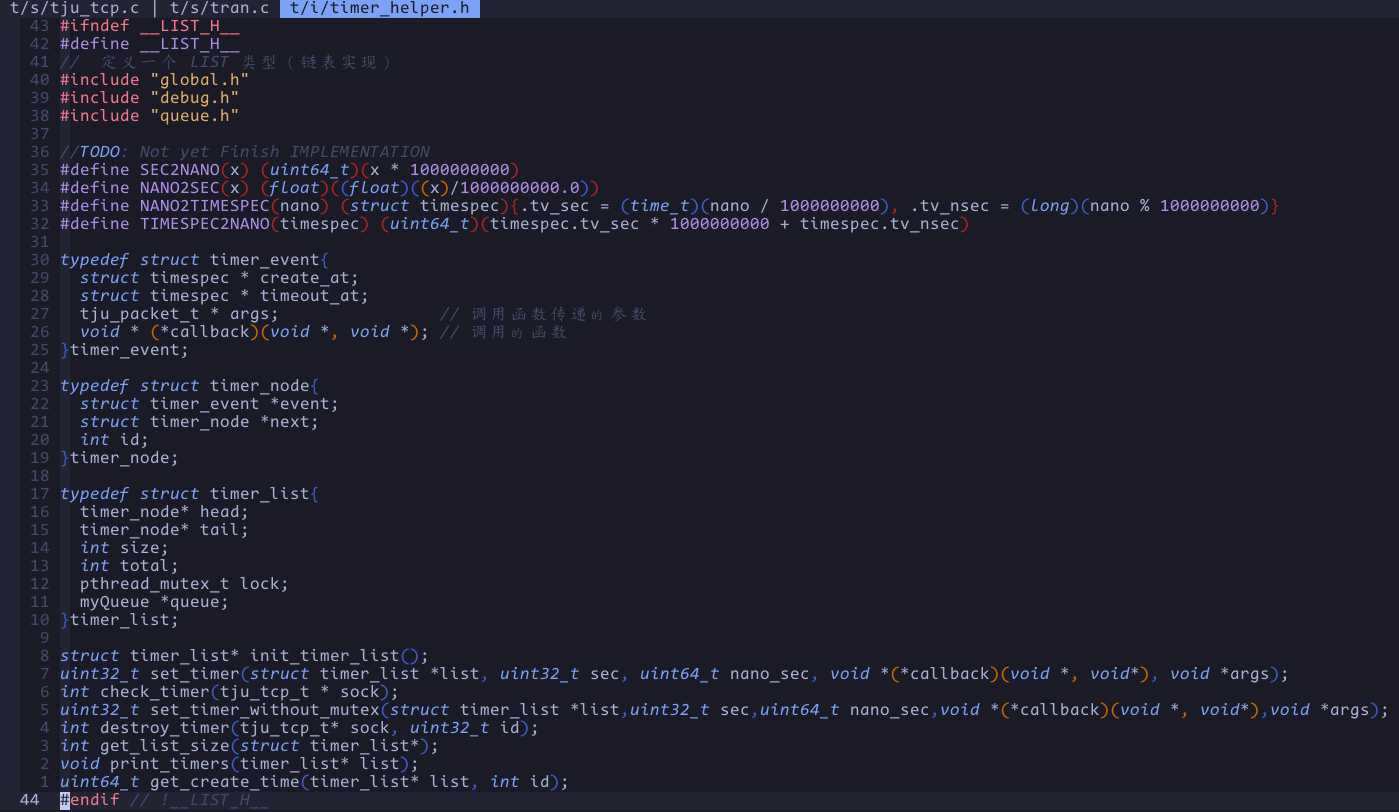
\includegraphics[width=1.0\textwidth]{timer_list.png}
    \label{fig:timer_list}\caption{timer\_list 数据结构}
  \end{figure}

\paragraph*{queue} 是对包括发送缓冲区、全连接队列以及清除队列(异步清除 timer )的具体实现。头文件如图\ref{fig:queue}所示。可以看到,我们使用 void* 表示当前结点装载的数据,这样实现的好处就是高扩展性,能够用来装载任何自定义的数据结构。缺点当然是使用不当会导致调用队列错乱。

\begin{figure}[!htbp]
    \centering
    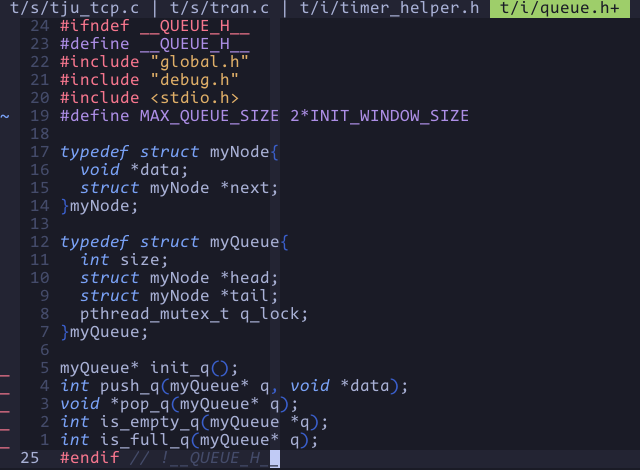
\includegraphics[width=0.9\textwidth]{queue.png}
    \label{fig:queue}\caption{queue 数据结构头文件}
  \end{figure}

  \begin{figure}[!htbp]
    \centering
    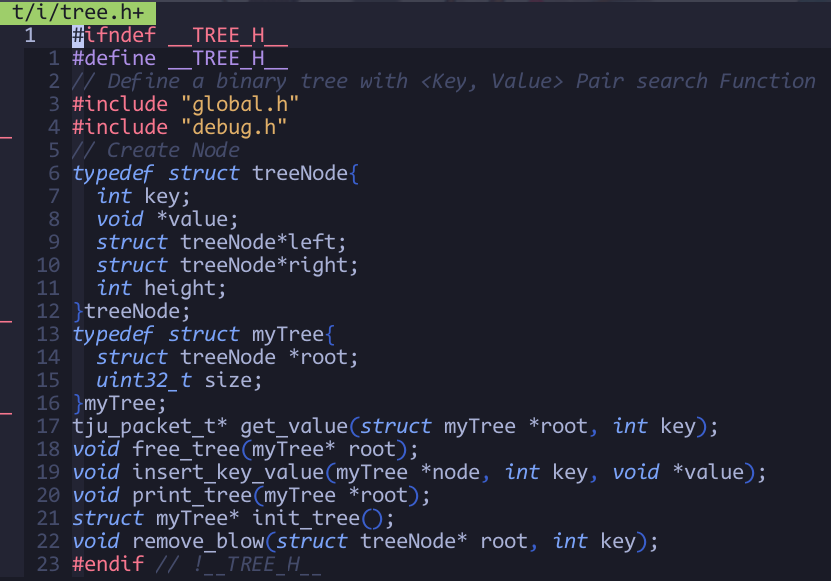
\includegraphics[width=0.9\textwidth]{tree.png}
    \label{fig:tree}\caption{tree 数据结构头文件}
  \end{figure}
  
\paragraph*{tree} 是对接收缓冲区的具体实现,在此我们采用了 AVL 的数据结构(自平衡搜索二叉树,aka 小根堆)。因为我们的应用场景是:存入乱序到达的包裹,并按照正序进行取出。使用 AVL 可将二者的操作时间复杂度降到 $log_2(N)$。图\ref{fig:tree}是 tree 的头文件。

\subsection{实现思想}

可靠数据传输的实现较为复杂。首先我们从发送线程的角度考虑,需要对发送的每个报文进行超时超时重传的检测。同时在接收到 ACK 后需要累计地将这些超时重传标签丢掉。

首先是在调用 tju\_send 时,按照原来的做法,是使用 send\_buf 进行发送。我们考虑到这个调用的流程逻辑本质上就是一种队列的思想:先从 tju\_send 进入发送队列的报文先发送。于是我们复用了半/全连接队列时创建的 QUEUE 数据结构,让 tju\_send 将报文放入 sending\_queue 中。再让发送线程通过 sending\_queue 取出需要发送的报文即可。

然后我们来处理超时重传:建立一个 timer\_list 结构,用于存放已经发送且未得到ACK的报文。在发送线程中,我们首先对这个 timer\_list 进行检查:按照顺序依次检查每个报文创建的时间和当前时间对比,如果有超时,则进行重发,否则直接退出。由于这个 timer\_list 特性,天然按照报文创建的时间进行排序,所以可以在第一次遇到不用重发时退出。

然后我们从接收写成的角度进行考虑:我们会接收到三种类型的报文:seq 小于、等于以及大于expected\_seq。所以我们的思路也就很明朗了:小于时将其丢弃,大于时将其放入之前定义的AVL树中,等于时将其放入 recv\_buf 并更新 expected\_seq,并在 AVL 树中按照 seq 的大小查找是否有乱序达到的报文。当然,三种情况都需要发送 ACK 回去通知收到。

\subsection{具体实现}

\paragraph*{Tju\_Send 实现} 在 Tju\_Send 中,首先需要判断上层内容的大小,若过大,则需要进行切片,以免在下层被切割。然后在进入阻塞状态,等待发送窗口出现空闲。然后交给发送窗口,同时调用发送函数,在 rwnd 的情况下将发送缓冲区的内容进行发送(此处在后期需要调整为 线程)

\paragraph*{Tju\_Recv 实现} 在 Tju\_Recv 中,首先进行阻塞等待,直到其他线程给接收缓冲区放入内容。待有内容后,再将内容 通过 Memcpy 提交给上层调用的实体。

\paragraph*{Socket 数据结构}
\begin{itemize}
    \item 给 window.wnd\_send 增加了 rwnd 和 cwnd 等控制发送的信息
    \item 给 window.wnd\_recv 增加了 AVL Tree 等数据结构,用于存放乱序到达的数据包
    \item 给 window.wnd\_send 增加了 rto 等字段,动态控制超时事件
    \item 给 window.wnd\_recv 增加了 expe\_seq 等字段,判断接收到的数据顺序正确与否
\end{itemize}

\subsubsection*{超时重传机制}

\paragraph*{超时重传定时器}
实现了 Timer\_Helpher 子系统,通过设置 set\_timer() 函数来新建一个 Timer,Delete\_timer() 来终止一个 Timer。使用了一个线程不断检查是否有超时的Timer,并进行重传和重置。使用 Mutex Lock 进行存储区域的一致性,使得在增加、删除和检查时只能有一个线程存在。

特别的,我们使用了链表的数据结构进行 Timer 的增加、删除和检查,链表能够高效地进行增加删除。同时,设置了 event 数据类型来处理当前 Timer 的超时操作(可以通过传入不同的函数和变量达到不同类型 Timer 的统一调用)。

\paragraph*{RTO调整}

由于我们每个需要重传的报文都对应一个 TIMER,所以我们能通过发送时的 Created\_At 和删除时的系统事件算出当前 Timer 提供的 sampleRTT 并 在每次进行 Timer 删除时,通过公式 \ref{eq:rto} 进行 RTO 的更新。

值得注意的是,这里依然需要大量使用 Mutex Locker 来控制:在更新 RTO 时,不能创建新的Timer,直到 RTO 更新完成。

\section{流量控制}

接收方发送ACK时,将自己缓冲区大小放入 advertised\_wind 字段。发送方在接收到 ACK 时,需要提取 rwnd 值。在设置发送窗口的大小时,我们需要考虑 rwnd(发送窗口大小), cwnd(拥塞控制), 以及自己本身的大小。

当得到 rwnd == 0 的情况时,发送方需要发送1比特的试探报文进行发送窗口的试探,同时需要设置超时机制进行不断试探。

\section{连接关闭的实现}

在实现连接关闭之前,我们需要统一说明一下目前 tju\_handle\_packet 中的 socket 状态种类,以便在后续的流程中解释更加清晰。

\paragraph*{连接建立} LISTEN, SYN\_SENT, SYN\_RECV, ESTABLISHED
\paragraph*{连接关闭} FIN\_WAIT\_1, FIN\_WAINT\_2, CLOSE\_WAIT, CLOSING, LAST\_ACK, TIME\_WAIT 

从代码实现的角度考虑,我们不需要在意当前情况是两方同时发起关闭还是一方先一方后。我们根据绘制的 FSM 图可以得出结论:我们根据 socket 状态以及接收到的报文进行状态的转换以及处理:

\begin{enumerate}
    \item \textbf{处于 ESTABLISHED 且发起 close} 发送 FIN 状态转化为 FIN\_WAIT\_1
    \item \textbf{处于 FIN\_WATI\_1 且收到 FIN 的 ACK} 状态转化为 TIME\_WAIT 超时后变为 CLOSED
    \item \textbf{处于 ESTABLISHED 收到 FIN} 状态变为 CLOSE\_WAIT 并返回 ACK 
    \item \textbf{处于 CLOSE\_WAIT 且发起 close} 状态转为 LAST\_ACK 且等待 ACK 
    \item \textbf{处于 LAST\_ACK 且收到 ACK} 状态转为 CLOSED 并关闭
\end{enumerate}

实现时需要注意的是,只要 socket 状态不是 CLOSED,都要继续接收新的报文并回复 ACK。

\section{拥塞控制的实现}

拥塞控制的实现核心在于两个事件触发拥塞窗口进行变化,且发送窗口随之而变。两个事件分别是:3个ACK,以及超时重传。

\paragraph*{3个ACK检测} 在 sock 中的 cwnd 数据结构中加入 last\_ack 以及 count 的整型数据,在 received\_ack 函数中对 last\_ack 进行比对并记录 count 是否增加或还原。

\paragraph*{超时检测} 在 check\_timer 中触发超时转换 cwnd 的大小。

需要注意的是需要创建一个 sshresh 对cwnd慢启动和拥塞避免进行转换。同时,需要记得在 3个ack后将状态调整为拥塞避免,在超时后将状态矫正为慢启动。


\section*{日志记录}

实现了日志 trace 模块,在Server Client 端调用 tju\_sock 的时候进行日志的初始化(即定义日志名,创建日志文件等)。然后通过提供的日志格式和事件,在相应事件发生时,调用响应函数进行日志的录入。




% !TEX root = ../tjumain.tex

\chapter{实验结果及分析}

\section*{实验测试环境}

通过 VirtualBox 虚拟机进行测试,脚本默认丢包率 6\%,延迟 6ms。系统环境如图\ref{fig:ubuntu} 所示。测试方法是使用脚本和修改后的测试脚本进行运行,分析输出的log进行debug。

\section{连接建立的功能测试与结果分析}

连接建立的Log文件如图\ref{fig:established_log}所示:

\begin{figure}[!htbp]
    \centering
    \subfigure[server 端]{\includegraphics*[width=0.45\textwidth]{e_server1.png}\label{fig:e_server}}
    \subfigure[client 端]{\includegraphics*[width=0.45\textwidth]{e_client1.png}\label{fig:e_client}}
    \caption{连接创建 Log }\label{fig:established_log}
  \end{figure}

可以看到,Client 端首先创建了第一个 SYN 报文并进行发送,然后由于初次设置的 Timer 并不合理,立马出现了 timeout,进行重传,在接收到 SYN | ACK 后确认建立全连接,并发送 ACK 同时删除一个 timer 。 Server 端接收到 SYN 报文后进行 SYN | ACK 的返回,最后接受到 ACK 后确定一个 Full Connection 的建立。

\section{可靠传输的功能测与结果分析}

\subsection{RTO动态调整}
如图\ref{fig:RTTFIG} 是在 100Mbps 20ms 延迟的情况下观测到的数据,可见,我们的 TimeoutInterval 的确是随事件变化、随EstimatedRTT变化的。

\begin{figure}[!htbp]
    \centering
    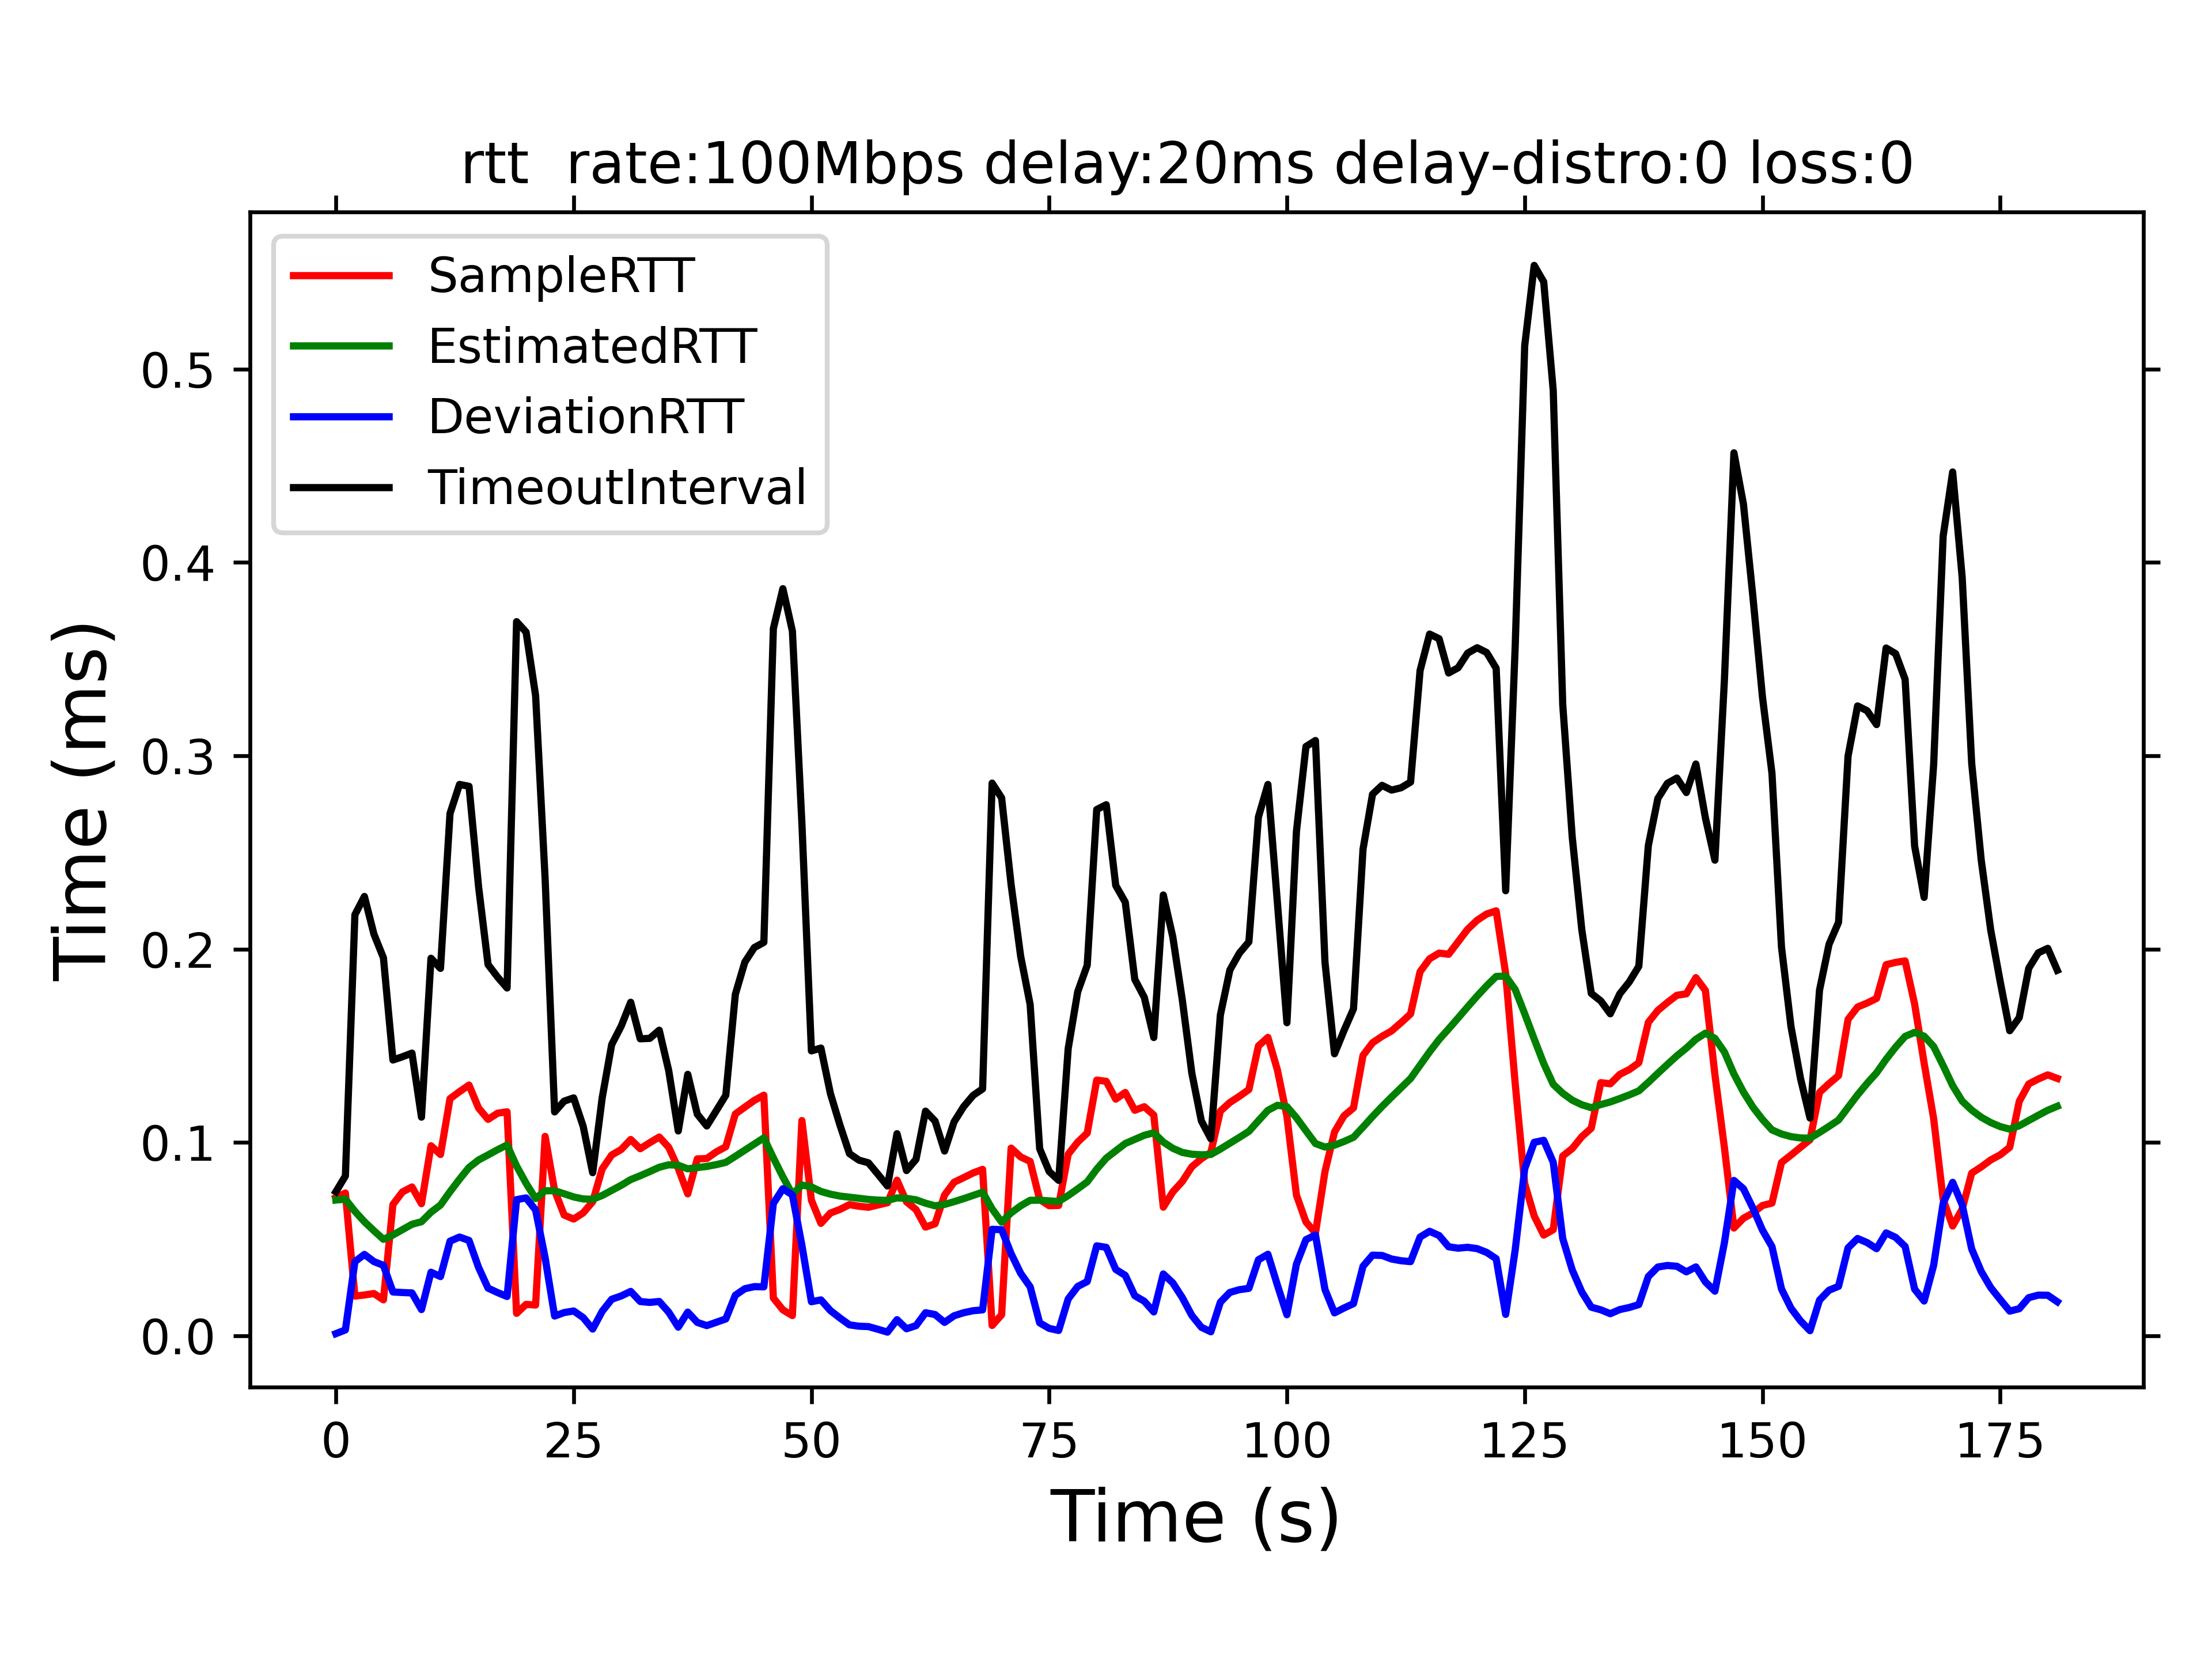
\includegraphics[width=5.5in]{RTT_FIG.png}
    \caption{RTT动态调整 图}\label{fig:RTTFIG}
\end{figure}

如图\ref{fig:RTTLOG}是 RTO 根据获得的 EstimatedRTT 进行的调整
\begin{figure}[!htbp]
    \centering
    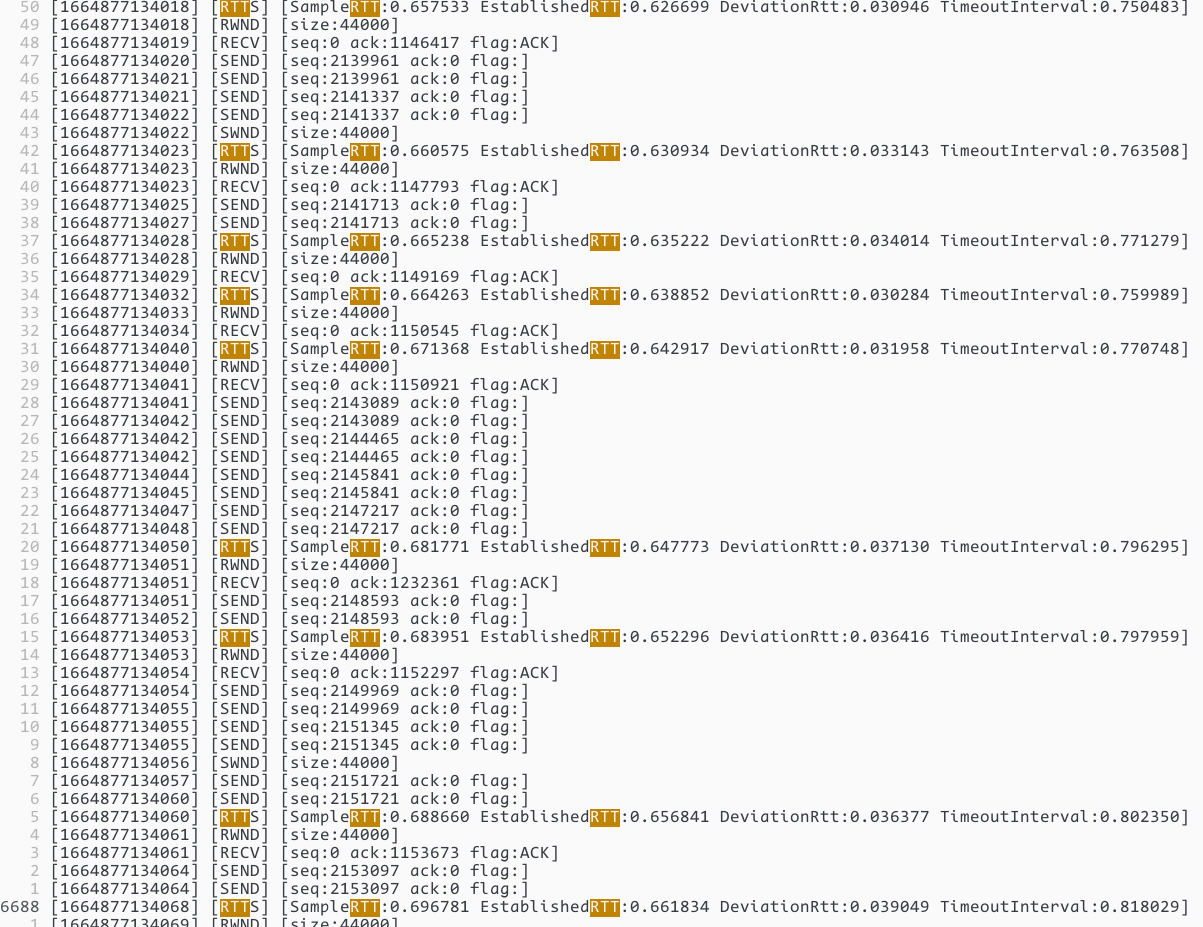
\includegraphics[width=5.5in]{RTT_LOG.png}
    \caption{RTT动态调整 Log}\label{fig:RTTLOG}
\end{figure}

\subsection{可靠数据传输}

我们通过 Client 端的 Trace (如图\ref{fig:recvLog})可以看到接受到连续 ACK 表明接收到了正确的信息。更多测试,在后续的性能中进行展示。

\begin{figure}[!htbp]
    \centering
    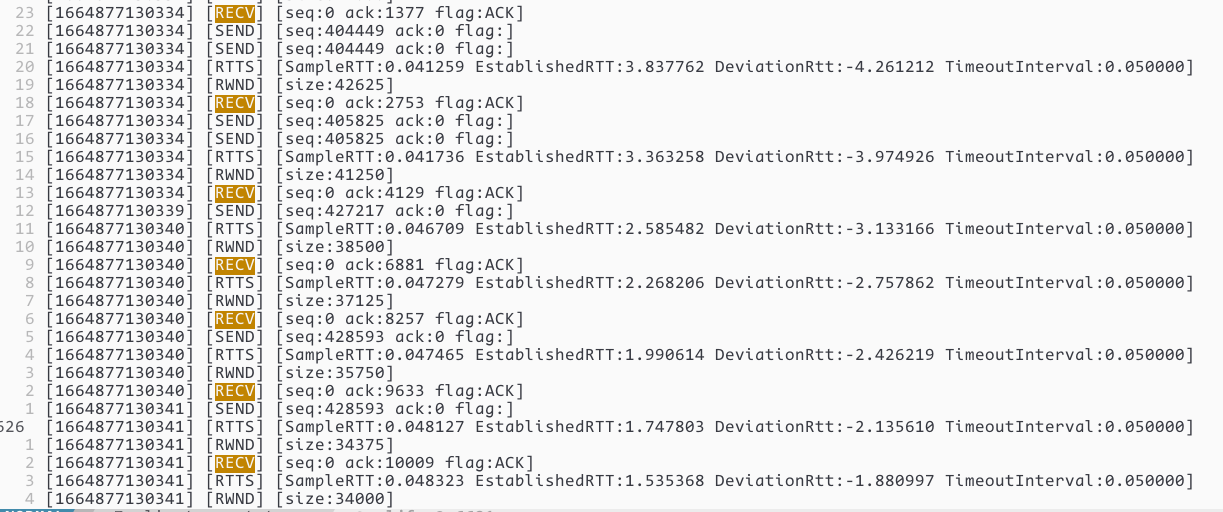
\includegraphics[width=5.5in]{RECV_LOG.png}
    \caption{接收 Seq 跟随变化图}\label{fig:recvLog}
\end{figure}

\section{流量控制的功能测试与结果分析}


为最大限度地选出优秀的结果,我们将家庭NAS服务器系统装上了 Arch Linux 并安装 vagrant 等进行大量脚本测试,跑出了 1728 个结果(如图\ref{fig:results_all}),精选后,我们选出一个较为优秀的结果精选展示。

\begin{figure}[!htbp]
    \centering
    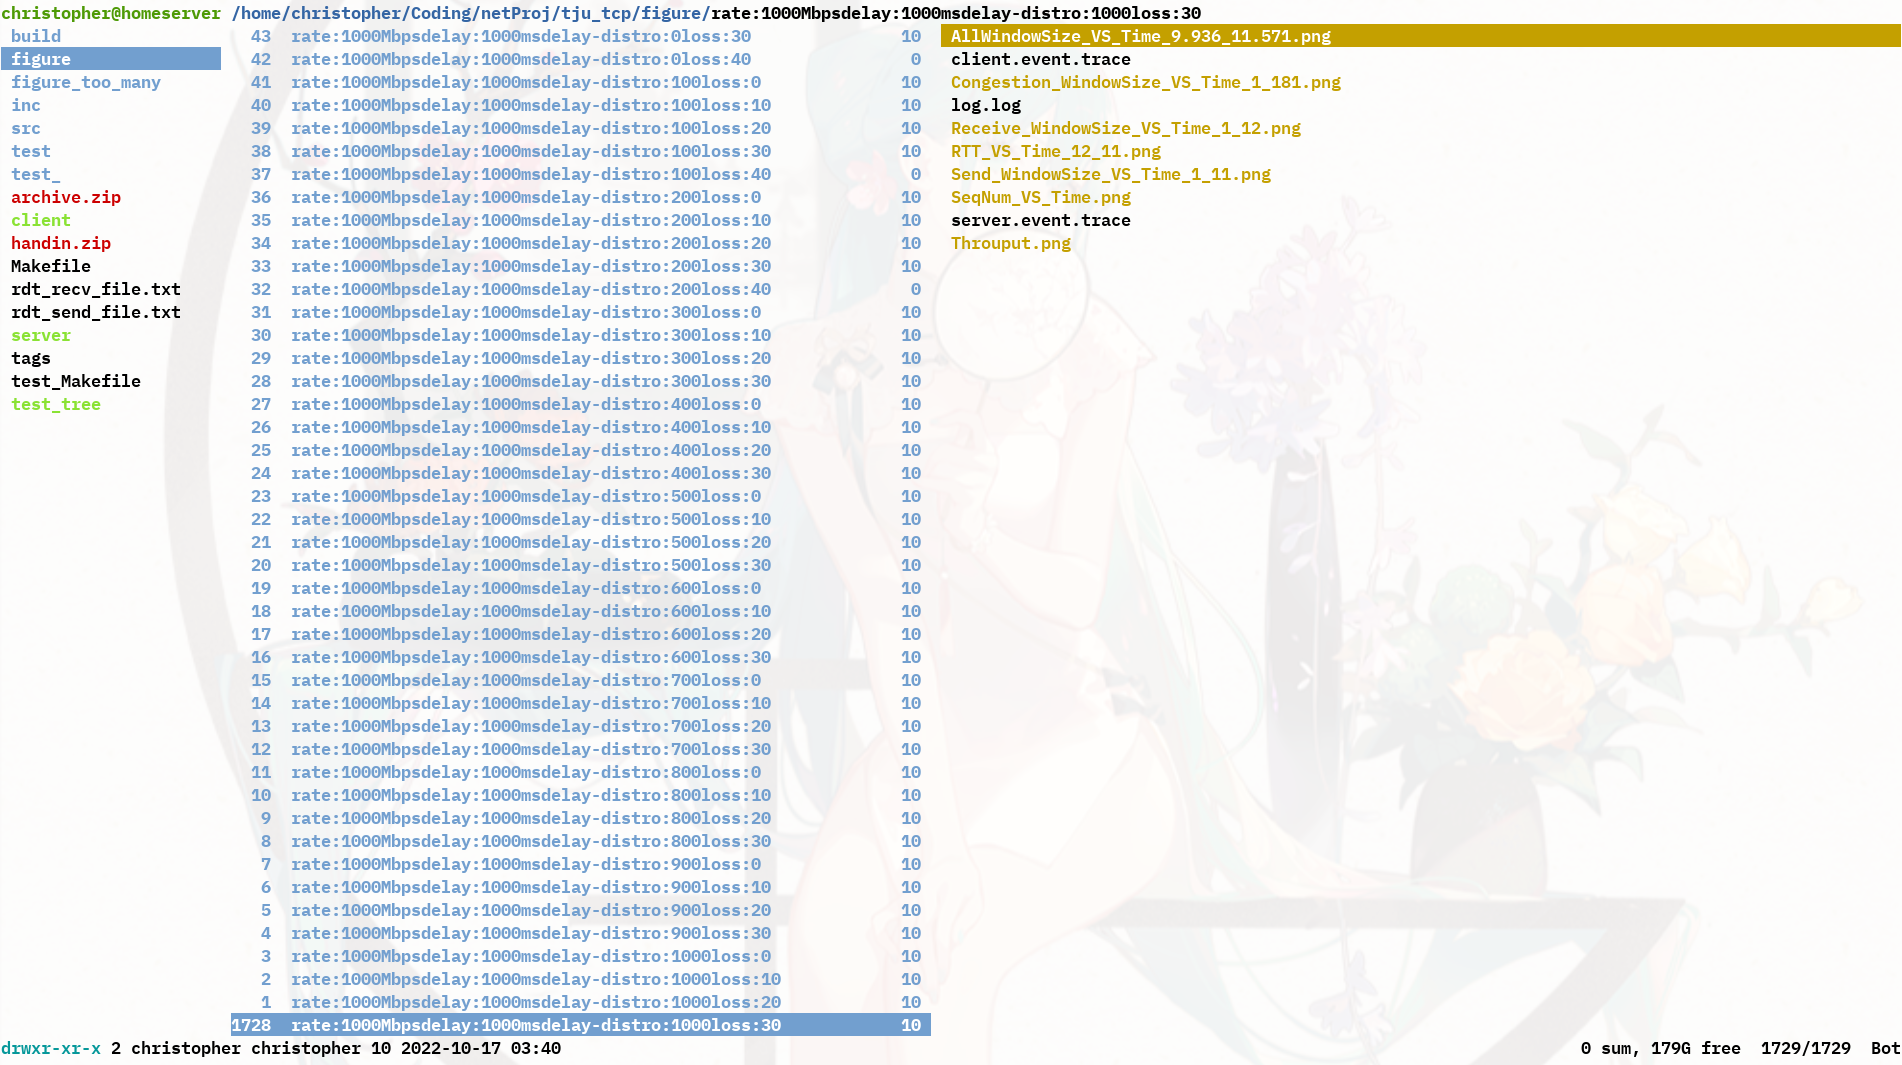
\includegraphics[width=5.5in]{homeserver.png}
    \caption{家庭NAS系统结果}\label{fig:results_all}
\end{figure}


我们选出在100Mbps 20ms 延迟环境下的测试结果\ref{fig:all_window}。显示我们的流量控制效果是合理的,能够将窗口的变化实时体现在 swnd 中。
\begin{figure}[!htbp]
    \centering
    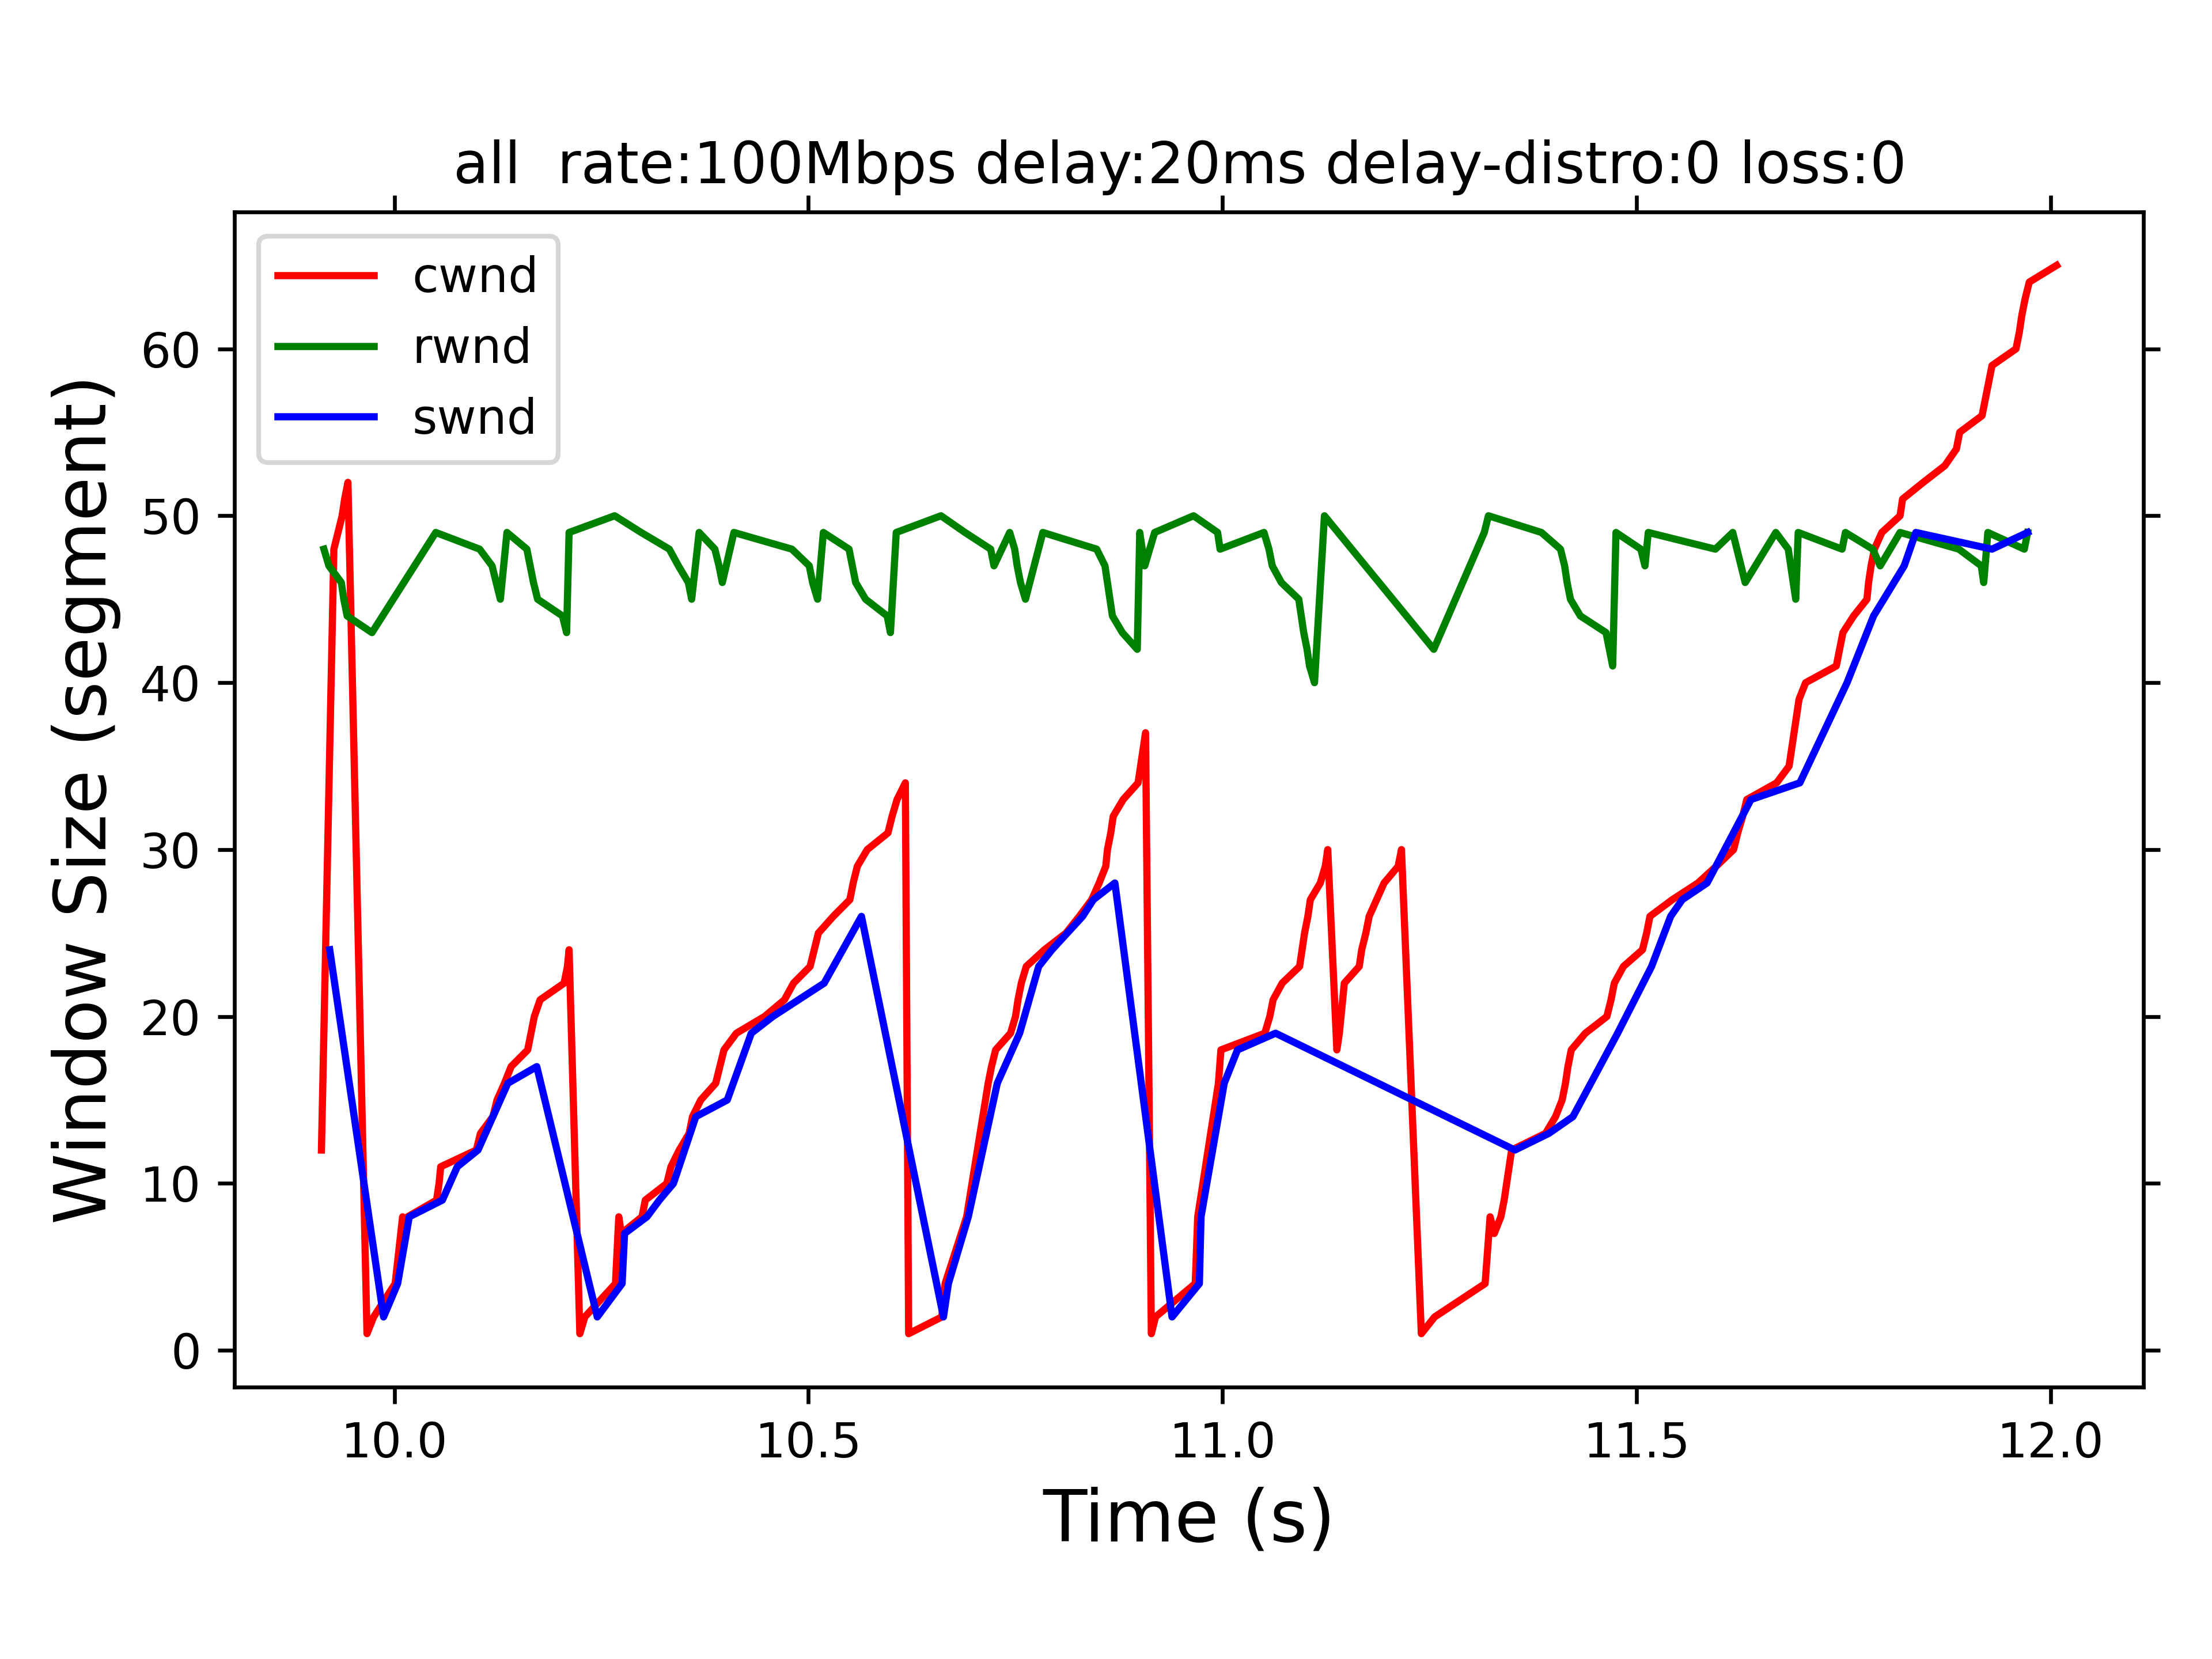
\includegraphics[width=5.5in]{all_window.png}
    \caption{流量控制}\label{fig:all_window}
\end{figure}

\section{连接关闭的功能测试与结果分析}
我们顺利在 Auto Lab 上提交了正确答案,确实没太多特性需要测试,在此附上一个 AutoLab上的截图证明(如图\ref{fig:close_test})。

\begin{figure}[!htbp]
    \centering
    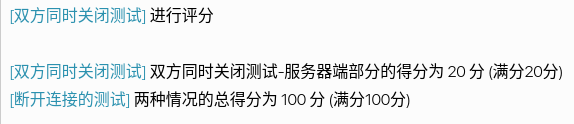
\includegraphics[width=4in]{close_test.png}
    \caption{连接关闭证明}\label{fig:close_test}
\end{figure}

\section{拥塞控制的功能测试与结果分析}
经过脚本测试,我们选出了在环境100Mbps 20ms延迟的数据进行展示,可以看到,我们的cwnd实现能够在正确地情况出现时给予正确的处理:即1. 刚开始时采取慢启动。2. 达到 sshresh 时采取拥塞避免。 3. 在发生超时的同时将窗口大小降低并进行慢启动。4. 出现三次 ack 时降低一般的窗口。整个图形呈现锯齿状

\begin{figure}[!htbp]
    \centering
    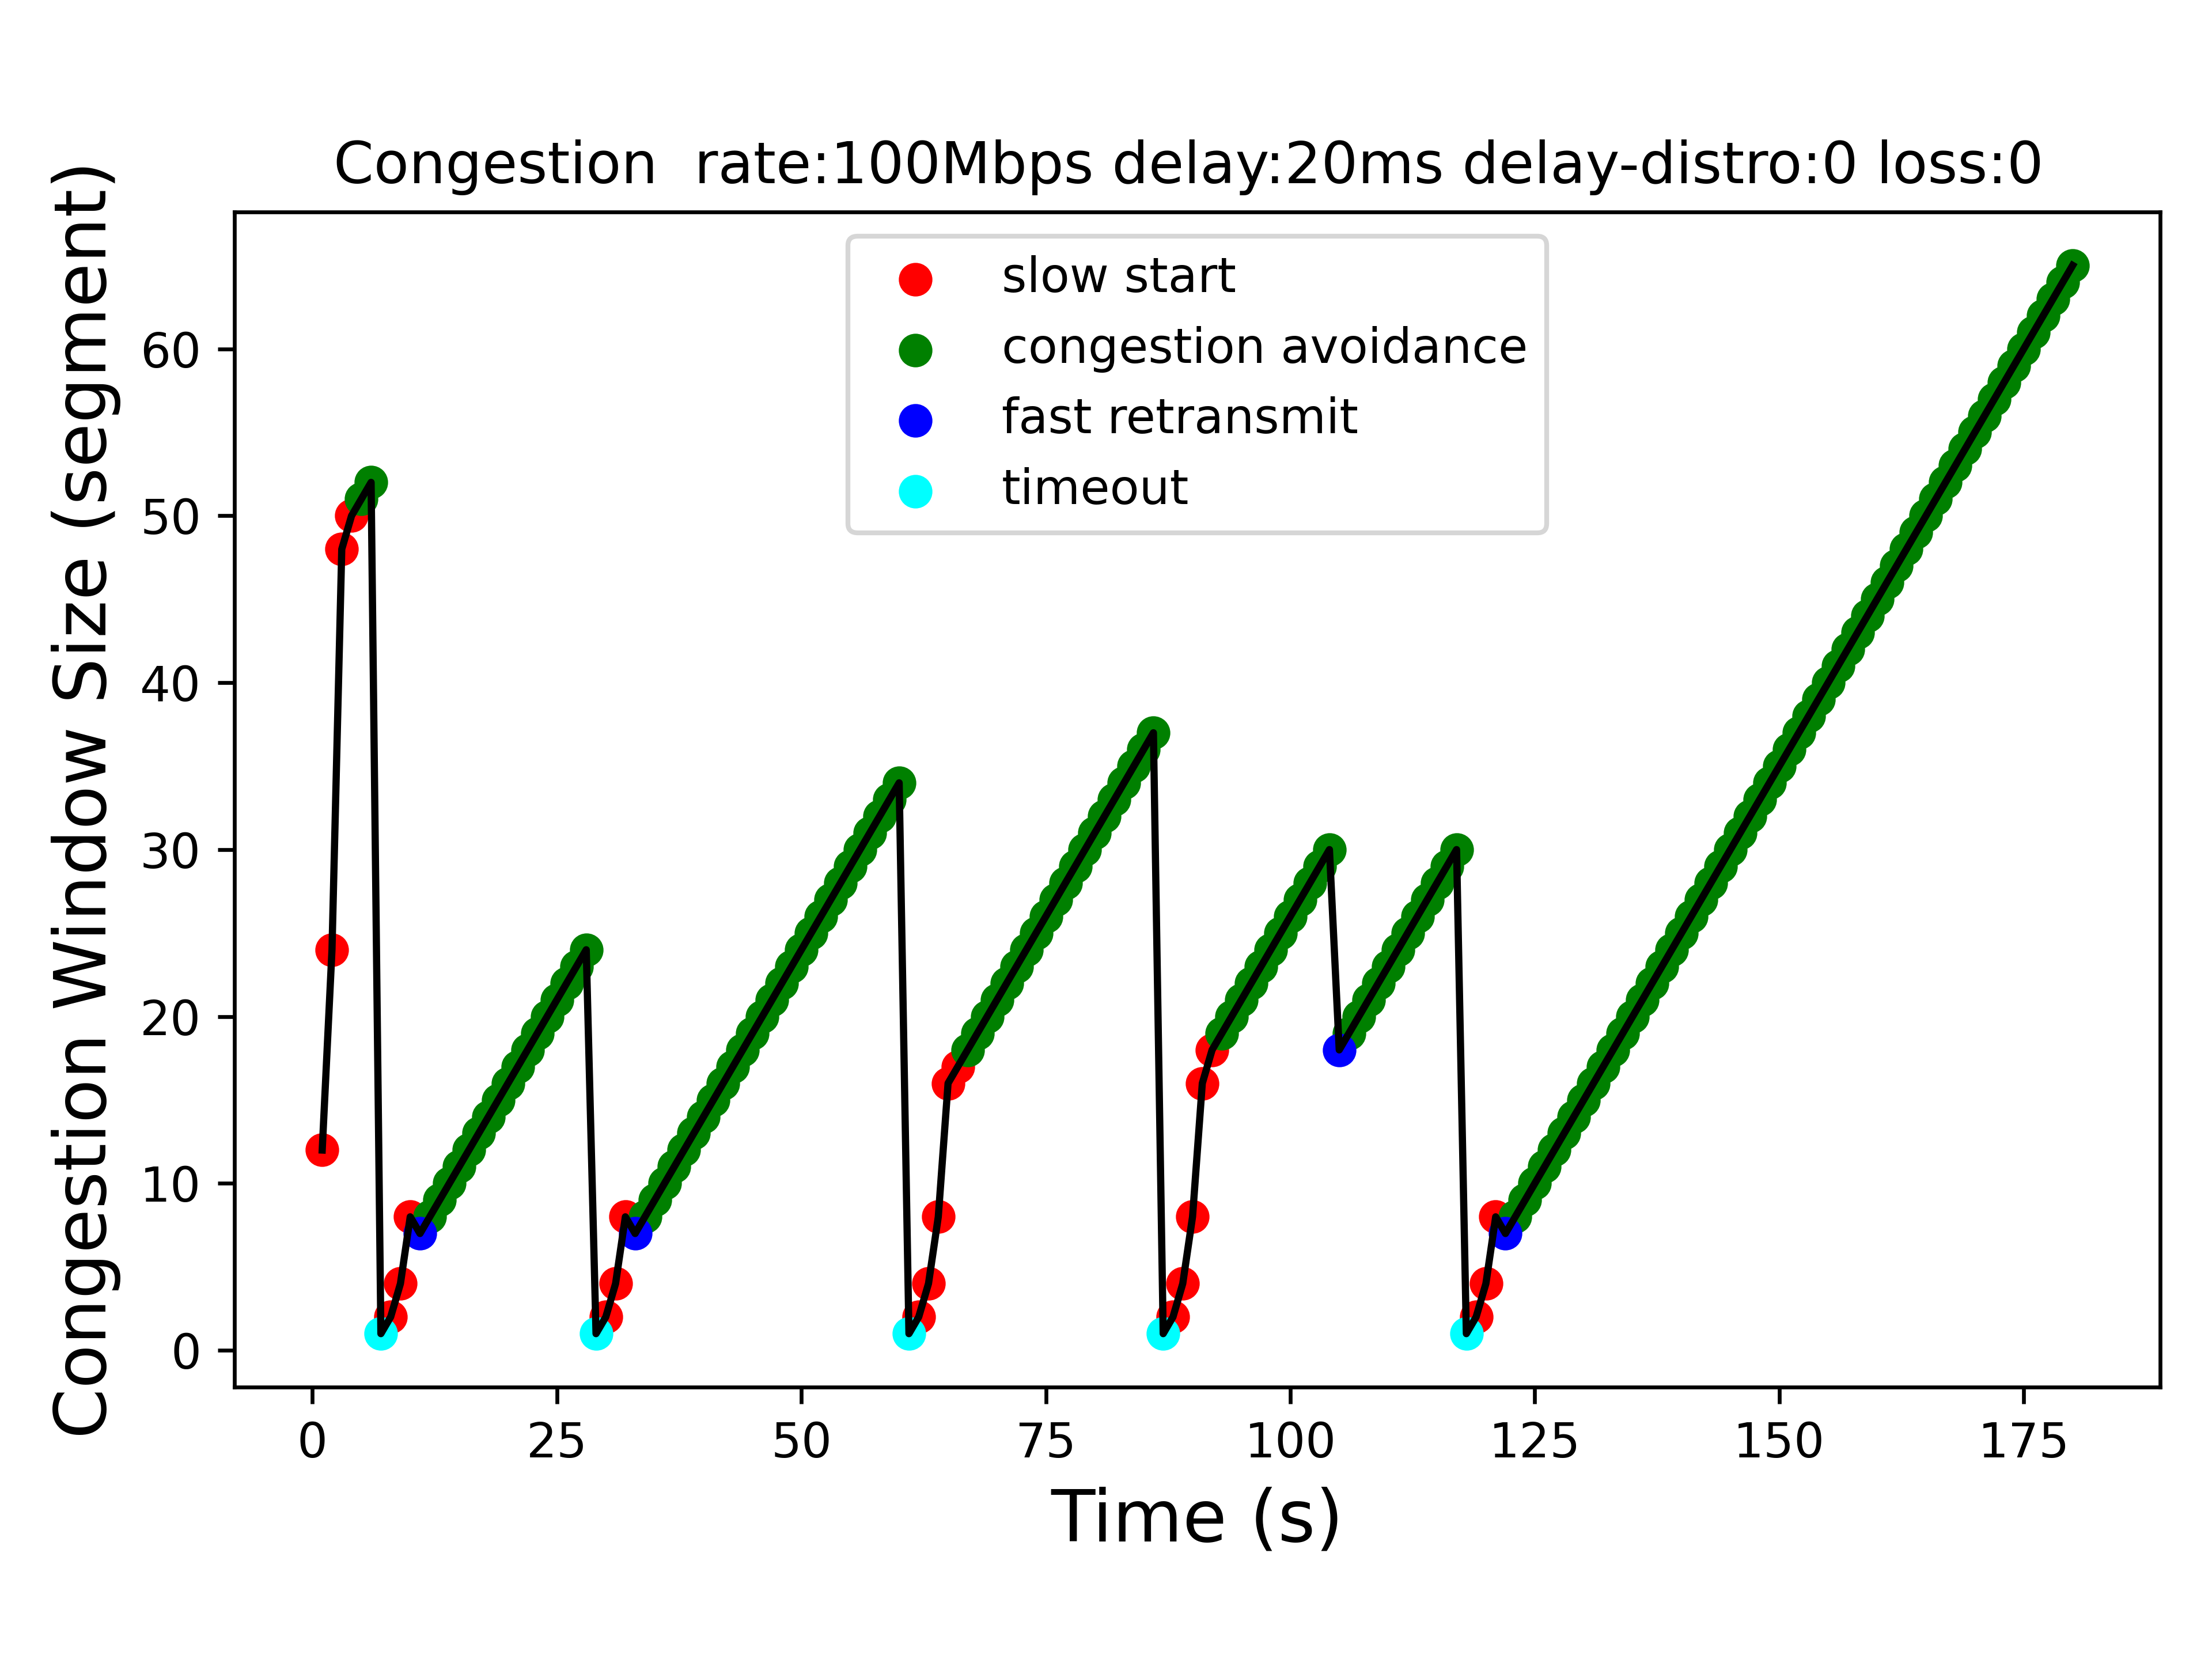
\includegraphics[width=5.5in]{conngestion.png}
    \caption{Congestion窗口变化图}\label{fig:congestion}
\end{figure}

\section{TCP协议性能测试与结果分析}

我们分别对吞吐率-窗口大小和吞吐率-丢包率两种情况做了测试(如图\ref{fig:throughtput-loss}和\ref{fig:throughtput-wds}所示)。

\begin{figure}[!htbp]
    \centering
    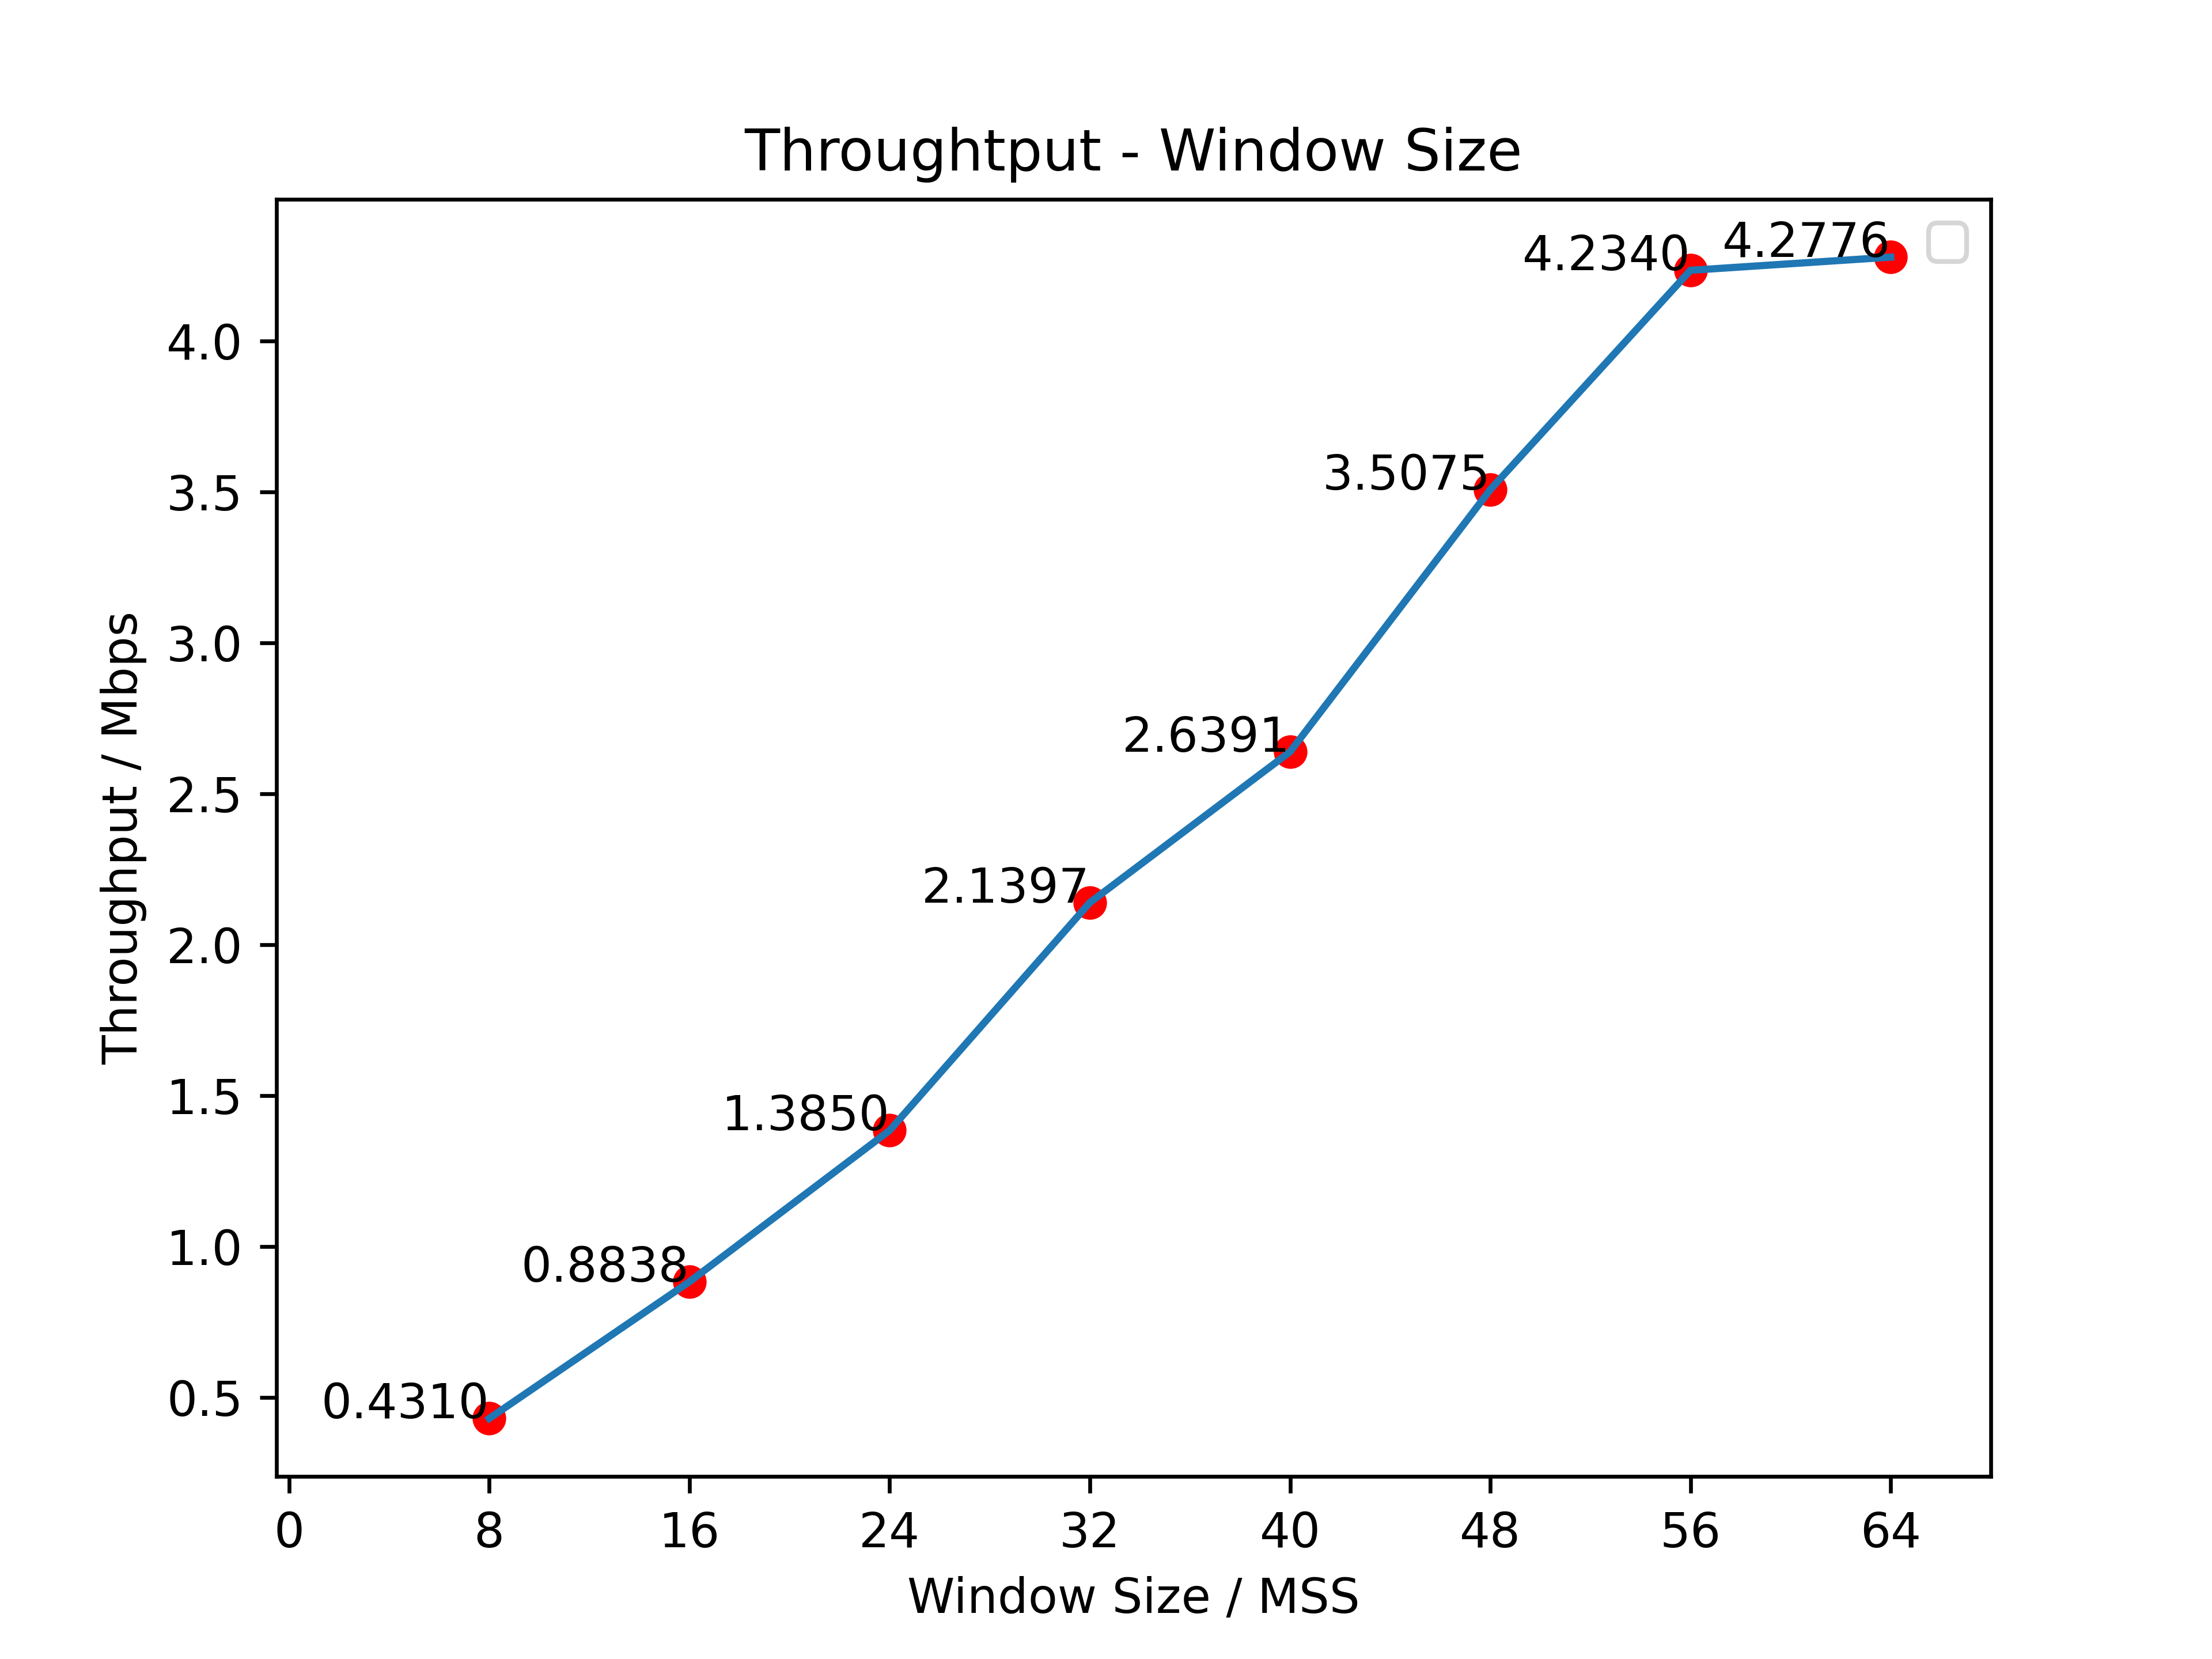
\includegraphics[width=5.5in]{wds.png}
    \caption{吞吐率-窗口大小}\label{fig:throughtput-wds}
\end{figure}


\begin{figure}[!htbp]
    \centering
    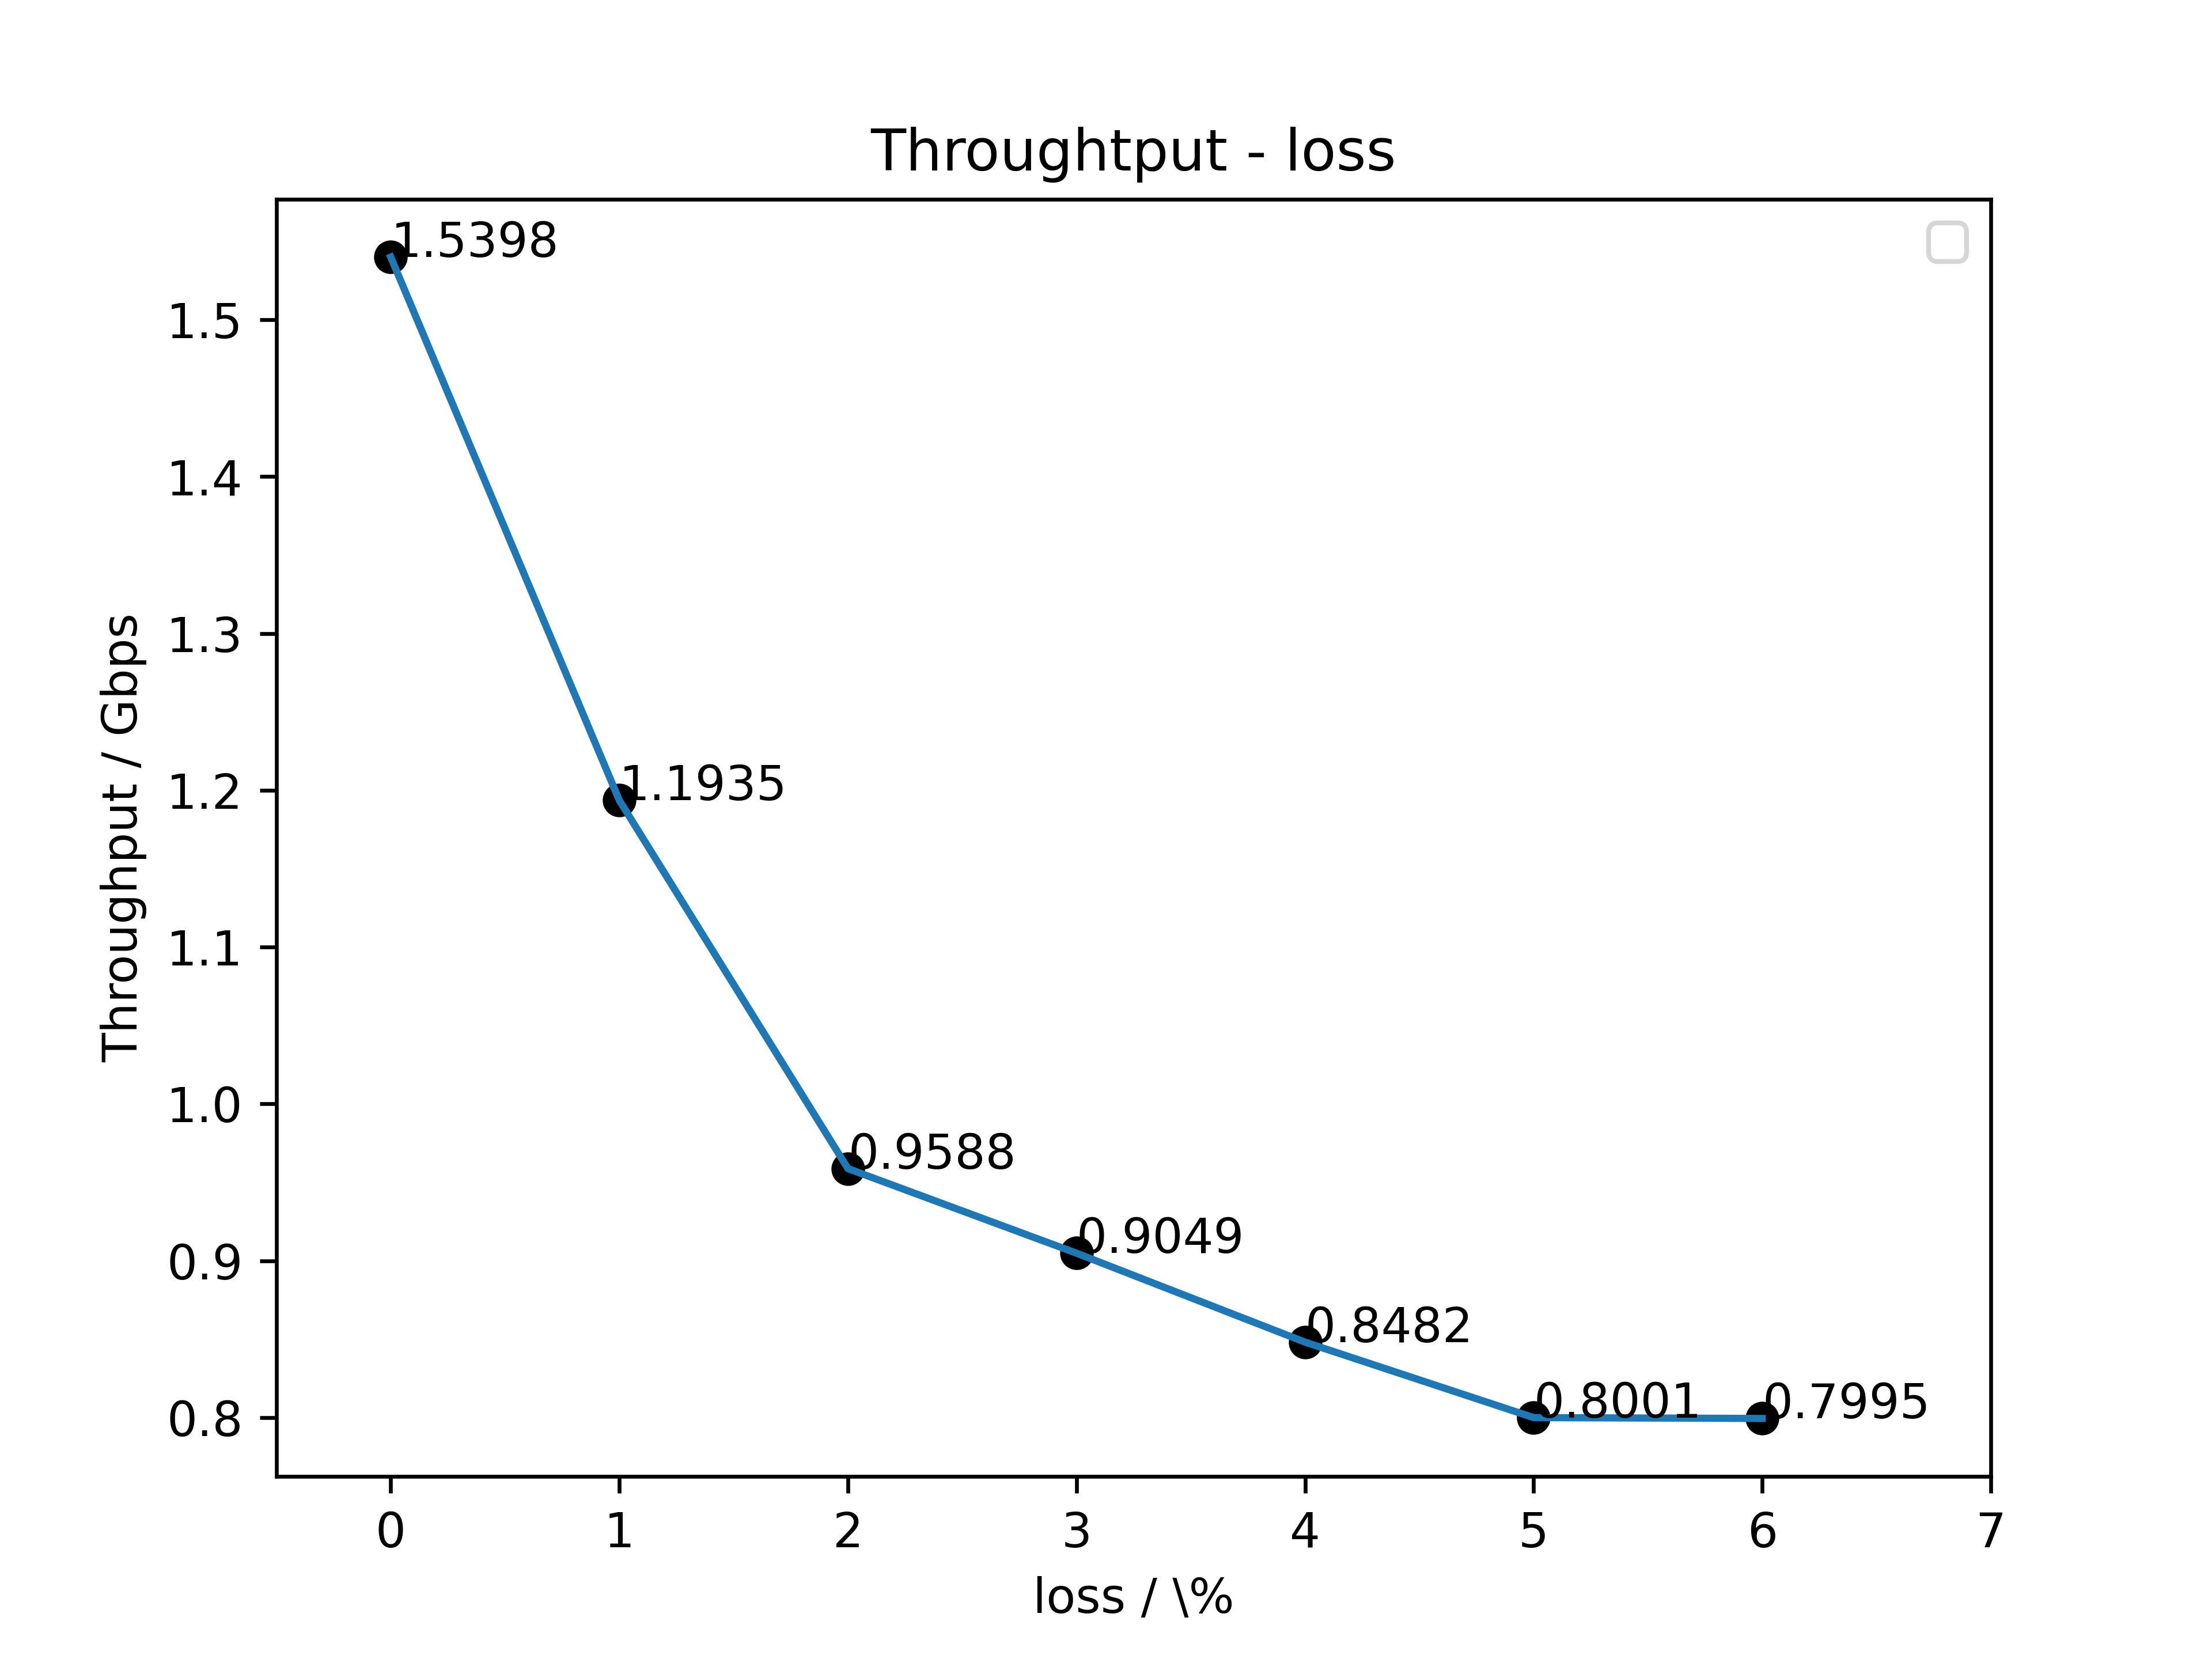
\includegraphics[width=5.5in]{loss.png}
    \caption{吞吐率-丢包率}\label{fig:throughtput-loss}
\end{figure}

\paragraph*{窗口大小} 可见,随着窗口大小的增加,吞吐率有明显地增大。但在较大的两个数据:56和64之间的吞吐率差距较小。这可能是因为我们仍然设置了对发送缓冲区的大小做了限制:即发送端在发送缓冲区满的时候需要停下来等待。且每次都需要对环境进行加锁、解锁,这些流程也会使得整体速率是有上限的。也就是说我们的表现是正确的。

\paragraph*{丢包率} 可见,吞吐率随着丢包率的提高而下降,我们选取的窗口大小为32,符合图\ref{fig:throughtput-wds} 的数据。同时,在产生1\%丢包率时,其吞吐率相较没有丢包率时有明显的下降。这表明在 TCP 现在的标准下,产生丢包等误判会严重降低吞吐率,我们或许有更好的设计思路能够提升这一情况下的吞吐率。






% \chapter{实验展示}


% \begin{figure}[htbp!]
%     \centering
%     \subfigure[Screemshot for Lab2.1]{\includegraphics[width=2.1in]{figures/wireshark1.png}}
%     \subfigure[Screemshot for Lab2.2]{\includegraphics[width=2.1in]{figures/wireshark2.png}}
%     \subfigure[Screemshot for Lab2.3]{\includegraphics[width=2.1in]{figures/wireshark3.png}}
%     \subfigure[Screemshot for Lab2.4]{\includegraphics[width=2.1in]{figures/wireshark4.png}}
%     \subfigure[Screemshot for Lab2.5]{\includegraphics[width=2.1in]{figures/wireshark5.png}}

%     \caption{Wireshak Application Screemshots}\label{fig:Wireshak Application Screemshots}
%     \vspace{-1em}
% \end{figure}

% \chapter{Q\&A}

% \section{The Basic HTTP GET/response interaction}



% \begin{enumerate}
%     \item Is your browser running HTTP version 1.0 or 1.1? What version of HTTP is the  server running?
    
%     \textbf{Answer:} Both are running HTTP version 1.1 
    
%     \item What languages (if any) does your browser indicate that it can accept to the server?
    
%     \textbf{Answer:} 简体中文(繁体),英文(US)。
    
%     \item What is the IP address of your computer? Of the gaia.cs.umass.edu server?

%     \textbf{Answer:}\\
%     My Computer: $172.23.170.212$\\
%     Server: $128.119.245.12$

%     \item What is the status code returned from the server to your browser?
    
%     \textbf{Answer:} Status Code: 200

%     \item What is the status code returned from the server to your browser?
    
%     \textbf{Answer:} Last-Modified: Sun, 13 Mar 2022 06:59:02 GMT

%     \item How many bytes of content are being returned to your browser?
    
%     \textbf{Answer:} 128 bytes

%     \item By inspecting the raw data in the packet content window, do you see any headers within the data that are not displayed in the packet-listing window? If so, name one.
    
%     \textbf{Answer:} No

% \end{enumerate}


% \section{The HTTP CONDITIONAL GET/response interaction}

% \begin{enumerate}
%     \item[8] Inspect the contents of the first HTTP GET request from your browser to the 
%     server. Do you see an “IF-MODIFIED-SINCE” line in the HTTP GET?

%     \textbf{Answer:} We see no "IF-MODIFIED-SINCE" line in the HTTP GET.

%     \item[9] Inspect the contents of the server response. Did the server explicitly return the 
%     contents of the file? How can you tell?

%     \textbf{Answer:} Yes, it did. We may see the whole HTML file in the content field. (Which shall be shown in the appendix section)

%     \item[10]  Now inspect the contents of the second HTTP GET request from your browser to 
%     the server. Do you see an “IF-MODIFIED-SINCE:” line in the HTTP GET? If 
%     so, what information follows the “IF-MODIFIED-SINCE:” header?

%     \textbf{Answer:} No we do see that line. Information: "Sun, 13 Mar 2022 06:59:02 GMT", which is same in the preview response, "Last-Modified" line.

%     \item[11] What is the HTTP status code and phrase returned from the server in response to 
%     this second HTTP GET? Did the server explicitly return the contents of the file? 
%     Explain

%     \textbf{Answer:} \textbf{Status Code: }304, \textbf{Phrase: }Not Modified.\\
%     The server did not explicitly return the contents of the file. Because the file is not modified since a specific time which makes it unnecessary to return too much information.

% \end{enumerate}

% \section{Retrieving Long Documents}

% \begin{enumerate}
%     \item[12] How many HTTP GET request messages did your browser send? Which packet 
%     number in the trace contains the GET message for the Bill or Rights?

%     \textbf{Answer:} 1 Get request was sent by my browser. The first one.

%     \item[13]  Which packet number in the trace contains the status code and phrase associated 
%     with the response to the HTTP GET request?

%     \textbf{Answer:} The first packet contains those informations. 

%     \item[14] What is the status code and phrase in the response?
    
%     \textbf{Answer:} \textbf{Status Code:} 200, \textbf{Phrase:} OK.
    
%     \item[15] How many data-containing TCP segments were needed to carry the single HTTP 
%     response and the text of the Bill of Rights?

%     \textbf{Answer:} There were 4 TCP segments in the HTTP response. Since it takes up for 4500 bytes and the first segment lasts for 1448 bytes, the text of the Bill of Rights takes up 4 segments (or 3 + $\frac{(4500-1448-14480-517)}{1448} = 3.75$ segments);

% \end{enumerate}


% \section{HTML Documents with Embedded Objects}
% \begin{enumerate}
%     \item[16] How many HTTP GET request messages did your browser send? To which 
%     Internet addresses were these GET requests sent

%     \textbf{Answer:} Totally there are 4 Get request messages. The IP Addresses are: "128.119.245.12"(First two), "178.79.137.164" and "221.81.63.166".

%     \item[17] Can you tell whether your browser downloaded the two images serially, or 
%     whether they were downloaded from the two web sites in parallel? Explain.

%     \textbf{Answer:} They are downloaded serially, since there is a "Connection: keep-alive" line and the time of each packet sent to the sever is strictly larger than the time recieving the response of the preview packet.

% \end{enumerate}


% \section{HTTP Authentication}
% \begin{enumerate}
%     \item[18] What is the server’s response (status code and phrase) in response to the initial HTTP GET message from your browser?
%     \textbf{Answer:} \textbf{Status Code:} 401, \textbf{Phrase:} Unauthorized;
    
%     \item[19] When your browser’s sends the HTTP GET message for the second time, what 
%     new field is included in the HTTP GET message?

%     \textbf{Answer:} \textbf{New Field:} "Authorization: Basic ..."
    
% \end{enumerate}



% \clearpage



% %%%%%%% 结论 %%%%%%%

% \addcontentsline{toc}{chapter}{Appendix: Annotation of the Output Files} %添加到目录中

% % \chapter*{Appendix}

